\documentclass[12pt,a4paper,ngerman]{scrartcl}

%% Laden der benoetigten Pakete:

\usepackage[utf8]{inputenc} %% West- & Mitteleuropa-Kodierung 

\usepackage{babel}% umfangreiches Sprachpaket (Silbentrennung, Gliederungen usw.)

\usepackage{graphicx}% Graphikpaket (fuer PNG,GIF,JPG)

\usepackage[caption=false]{subfig}% Mehrfachabbildungen

\usepackage{float,rotating}%Option [H] fuer fixe Position; Drehung von Abbildungen etc.

\usepackage{array,booktabs}%erweiterte Moeglichkeiten zur Tabellendarstellung

\usepackage{capt-of}

\usepackage{subfig}

\usepackage{wrapfig} %Einbetten von Bildern, Tables etc. in den Text ermöglichen

\usepackage{cite} %Zitieren nach IEEE mit dem Befehl \cite{bla} auf Refrent in thebibliography mit kennung "`bla"'

\usepackage{float} % Bei Gleitobjekten Position mit [H] festsetzen! (Sparsam verwenden!)
%
\usepackage{tikz}%Mindmaps etc.
\usetikzlibrary{mindmap,backgrounds}

% fix citations to be IEEE style
\def\citepunct{], [}
\def\citedash{]--[}

\usepackage{amsmath,amssymb,amsfonts,amsthm}% American Mathematical Society Pakete
\usepackage{textcomp,gensymb}% umfangreiche Pakete fuer Symbole wie:
%% \textmu, \textcelsius, \micro, \ohm, \degree, \celsius
%Kürzen in formeln
\usepackage{cancel}
%Farben ermöglichen
\usepackage{color} 

%\multirow ermöglichen in Tabellen
\usepackage{multirow} 

%Römische Zahlen mit  \RM{}
\newcommand{\RM}[1]{\MakeUppercase{\romannumeral #1{.}}}


%Bessere Worttrennung, Kerning ein. 
\usepackage[protrusion=true,expansion=true, kerning]{microtype}

%% Bildunterschriftengestaltung:
\addtokomafont{caption}{\footnotesize}
\addtokomafont{captionlabel}{\bfseries}
\usepackage[pdftex]{hyperref}

\newtheorem{bsp}{Beispiel}[section] %Beispielumgebung, zählschema: Kapittelnummer.Beispielnummer

\setcapwidth[l]{1\linewidth} %Captions unter Tabellen, Bildern etc. Linksbündig und wenn nötig die gersame Seitenbreite

%Einzelzeilen oben und unten unterbinden ("`Hurenkinder"' und "`Schusterjungen"')
\clubpenalty = 10000
\widowpenalty = 10000 
\displaywidowpenalty = 10000

%% Kopf- und Fusszeilengestaltung:
\usepackage{fancyhdr}
\pagestyle{fancy}%Seitenstil mit Kopf- und Fußzeilen
%\lhead{Modul 2} % MODUL O.Ä. HIER EINTRAGEN
%\chead{Gruppe 2}  % GRUPPE, NAME O.Ä. HIER EINTRAGEN
\rhead{Seite \thepage} \lfoot{} \cfoot{} \rfoot{} %Seitenzahlen in Header ausgeben
\renewcommand{\headrulewidth}{0.2pt} %Größe der Kopfzeile

%Dokumentinformationen 

\author{William Glover}
\title{Systemtheorie und Regelungstechnik} 

%% Layout-Umdefinitionen für die Titelseite (Zum benutzen Kommentierungen mit % vor den Kommandos entfernen) Umdefinition für das restliche Dokument findet an anderer Stelle statt!

% \renewcommand{\baselinestretch}{1.5} %1.5facher Zeilenabstand
% \renewcommand{\labelitemi}{-} %Spiegelstriche statt Bullets

%% Gestaltung der Titelseite:
\renewcommand\maketitle{
    \begin{titlepage}
        \sffamily
        \thispagestyle{empty}
              
\includegraphics[height=2.5cm]{IMTEK_Logo_Farbe}\hfill
\includegraphics[height=3cm]{Uni_Siegel}
        \par
        \vspace{2cm}
        \begin{center}
            \Huge \textbf{Mitschrieb der Vorlesung ``Systemtheorie und Regelungstechnik''}\\
            (SS 2010)\\[6cm]
            \end{center}
            %\includegraphics[height=7cm]{Bla} % BILD AUF DECKBLATT HIER EINBAUEN 
           
% Tabellarische Auflistung der wichtigen Daten des nachfolgenden Werkes. Nach belieben anpassen.

            \begin{tabular}{l}
                \large Dozent: Dr.-Ing. A. Peter\\
         \end{tabular}
         \\
						\begin{tabular}{ll}
                \large Textsatz von William Glover \\
                \large Stand: \today
            \end{tabular}
        
        
%Leere Seite, damit Inhaltsverzeichnis nicht auf der Rückseite des Deckblattes.(Bei Druckversion, bei Emailabgabe auskommentieren!)

 			 \newpage 
       \thispagestyle{empty}~
       \newpage

%Ende leere Zwischenseite   
 
\end{titlepage}
}

%% Liste fuer Silbentrennung bei komplexen Woertern:
\hyphenation{reibungslos schluss-endlich realisiert ter-min-liche}

%% Layout-Umdefinitionen:
\renewcommand{\baselinestretch}{1.5} %1.5facher Zeilenabstand
% \renewcommand{\labelitemi}{-} %Spiegelstriche statt Bullets
\setlength{\parindent}{0pt} % kein Erstzeileneinzug
\begin{document}
\maketitle %Titelseite setzen
\clearpage %danach neue Seite
\renewcommand{\baselinestretch}{1.5} %1.5facher Zeilenabstand
\thispagestyle{empty} %Header auf Titelseite unterdrücken

\tableofcontents %Inhaltsverzeichnis setzen
\newpage 

%Leere Seite, damit Inhalt nicht auf der Rückseite des Inhaltsverzeichnisses beginnt. (Bei Druckversion, bei Emailabgabe auskommentieren!)
        
        \thispagestyle{empty}~
        \newpage
     
%Ende leere Zwischenseite

\setcounter{page}{2} %Seitenzahl auf 2 setzen

% AB HIER BEGINNEN DIE INHALTE!

\addtocounter{section}{-1}%Counter einstellen, sodass Vorwort Kapitel 0 ist.
\section{Vorwort}

\begin{description}
\item[Systemtheorie, Kybernetik:] Allgemeine, formale Wissenschaft von der Struktur, den Relationen und dem Verhalten dynamischer, insbesondere komplexer Systeme, die gewisse allgemeine Eigenschaften realer Systeme aus den verschiedenen Bereichen der Wirklichkeit widerspiegeln. 
\end{description}

\subsection*{Ziele}

\subsubsection*{Beschreibung dynamischer Systeme}
\begin{description}
\item[Methoden:] Modellierung (z.B. als Blockschaltbild, DGL oder Übertragungsfunktion), Simulation (kostengünstig, ungefährlich), ...
\end{description}

\subsubsection*{Analyse dynamischer Systeme}
Fragestellungen wie z.B. ist das System...
\begin{itemize}
\item ...stabil?
\item ...steuerbar?
\item ...schwingungsfähig?
\end{itemize}

\subsubsection*{Beeinflussung dynamischer Systeme}
Ziel der Systemtheorie ist ein \emph{automatisierter, sicherer, optimaler Betrieb von technischen Systemen}. Dies kann auf zwei Arten erreicht werden
\begin{itemize}
\item \textbf{Regelung (kont. Systemzustände):} Ansteuerung des Systems, sodass die Ausgangsgröße den gewünschten Sollverlauf erreicht
\item \textbf{Steuerung (diskrete Systemzustände):} Bei gestörten oder zum Teil unbekannten Systemen fortlaufende Systembeobachtung und Rückführung.
\end{itemize}

\section{Beschreibung dynamischer Systeme durch das Blockschaltbild (BSB)}

\subsection{Beispiele zum Aufstellen eines BSB}
\begin{bsp}[Füllen eines Behälters]
\end{bsp}
\begin{figure}[H]%In Figure einpacken, damit am ENde der Minipageumgebung genug Abstand zum folgenden Text gelassen wird
\begin{minipage}{0.4\linewidth} 
 \begin{figure}[H]
  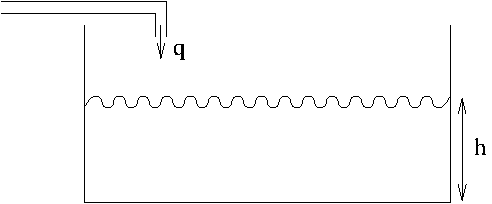
\includegraphics[width=\linewidth]{sysregel_bsp_1} 
  \end{figure}
\end{minipage}
\begin{minipage}{.6\linewidth}
$q(t):\text{Zufluss}$\\
$h(t):\text{Füllstand}$\\
$A:\text{Grundfläche des Behälters}$
\end{minipage}
\end{figure}
Lässt sich hier eine Gesetzmäßigkeit erkennen? Ja! Volumenbilanz:
\begin{equation*}
 v(t)= A \cdot h(t)=\int_0^t{q(\tau)d\tau}(+v_0) 
\end{equation*}
$v_0$: Volumen zum Zeitpunkt $t=0$ \\$\Rightarrow \text{für } v_0 = 0$ gilt:
\begin{equation*}
h(t)=\frac{1}{A}\int_0^t{q(\tau)d\tau}
\end{equation*}
Diese Abhängigkeit lässt sich als ein sogenanntes \emph{Blockschaltbild} wie folgt darstellen:
\begin{figure}[H]
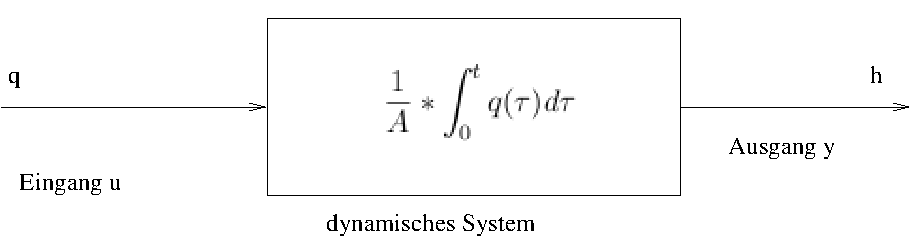
\includegraphics[width=9cm]{sysregel_bsb1}
\end{figure}
Es ist naheliegend, für übliche Operationen eine Bibliothek mit Standard-Blöcken anzulegen, im hier betrachteten Fall z.B. das sogenannte \emph{Integrierglied} (I-Glied).
Die allgemeine Integrationsfunktion
\begin{equation*}
  y(t)=k*\int_0^t{u(\tau)d\tau}
\end{equation*}
wird durch den folgenden Standardblock beschrieben:
\begin{figure}[H]
  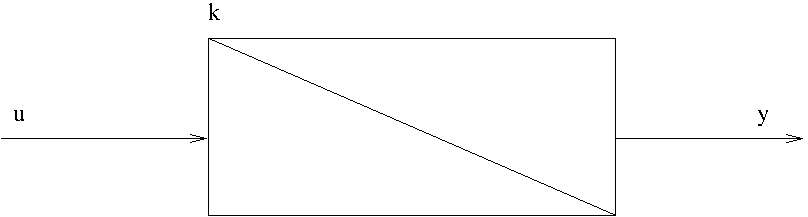
\includegraphics[width=7cm]{sysregel_iglied}
\end{figure}
\begin{bsp}[Erweiterung des Behälters um einen Ablauf]
\end{bsp}
\begin{figure}[H]
\begin{minipage}{0.4\linewidth}
\begin{figure}[H]
  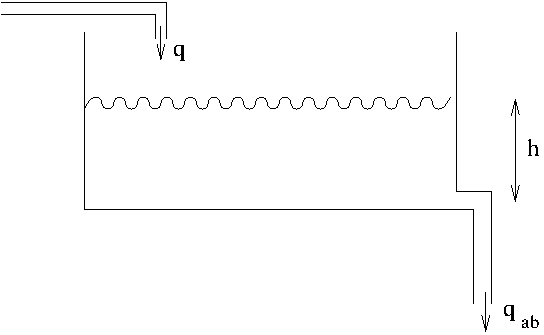
\includegraphics[width=.9\linewidth]{sysregel_bsp_2}  
\end{figure}
\end{minipage}
\begin{minipage}{0.6\linewidth}
$\begin{array}{lll}
q(t)&:&\text{Zufluss}\\
h(t)&:&\text{Füllstand}\\
A&:&\text{Grundfläche des Behälters}\\
q_{ab}(t)&:&\text{Abfluss}
\end{array}$
\end{minipage}
\end{figure}
Für diesen erweiterten Fall wird erneut die Vulumenbilanz aufgestellt:
\begin{equation*}
 v(t)= A \cdot h(t)=\int_0^t{q(\tau)-q_{ab}d\tau}=\int_0^t{u(\tau)d\tau} 
\end{equation*}
Diese lässt sich unter der Annahme, dass $q_{ab}$ von der aktuellen Füllhöhe abhängt, erneut in einem Blockschaltbild folgendermaßen darstellen:
\begin{figure}[H]
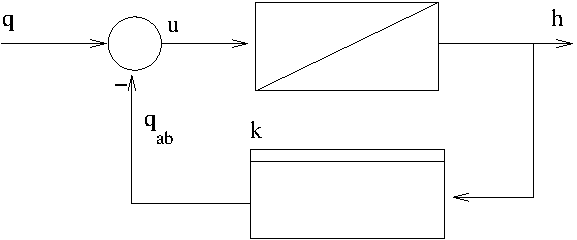
\includegraphics[width=7cm]{sysregel_bsb2}
\end{figure}
Hier wurden bereits zwei weitere, wichtige Standardblöcke eingeführt:
\begin{figure}[H]
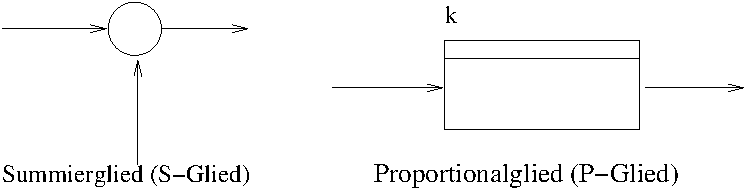
\includegraphics[height=2.5cm]{sysregel_spglied}
\end{figure}
Anhand des Blockschaltbild erkennt man sehr leicht, dass der Füllstand $h(t)$ sich nach einer gewissen Zeit nicht mehr ändert. Der aktuelle Füllstand wird zurückgeführt und vor der Integration von $q(t)$ abgezogen. Sobald gilt $q_{ab}=q$, bleibt $h(t)$ konstant. $u(t)$ wird Null (Stationärer Zustand)!

Da das beschriebene Systemverhalten sehr häufig vorkommt, wird dieses Blockschaltbild zu einem eigenen Standardblock zusammengefasst:
\begin{figure}[H]
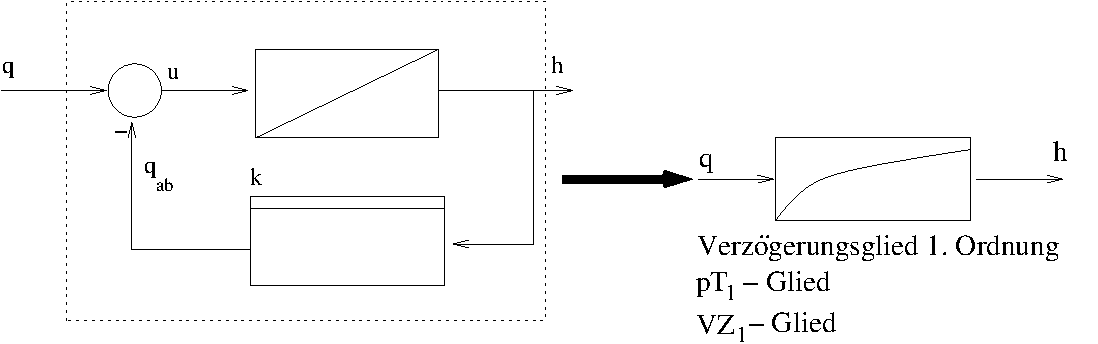
\includegraphics[height=4cm]{sysregel_pt1}
\end{figure}

\begin{bsp}[RC-Glied]
\end{bsp}
\begin{figure}[H]
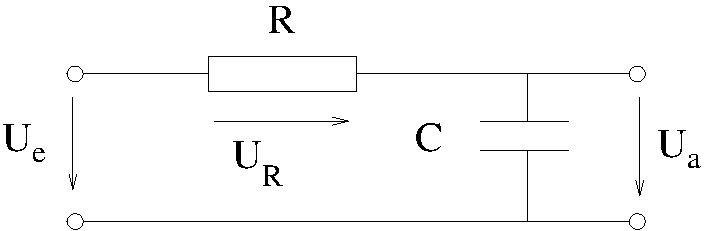
\includegraphics[height=2.5cm]{sysregel_RC}
\end{figure}
Das abgebildete RC Glied wird durch die Gleichungen
\begin{align*}
  \begin{array}{lrlll}
  U_a(t)&=&&\frac{1}{C}*\int_0^t{i(\tau)d\tau}\\
  U_e&=&&U_R+U_a &\Rightarrow U_R=U_e+U_a\\
  \rightarrow i&=&&\frac{U_R}{R}\\
  \Rightarrow i&=&&\frac{1}{R}(U_e-U_a)
 \end{array}
\end{align*}
beschrieben. Für $U_a$ ergibt sich daraus die Gleichung
\begin{equation*}
  U_a(t)=\frac{1}{RC}*\int_0^t{U_e(\tau)-U_a(\tau)d\tau}
\end{equation*}
Auch diese Funktion wird anschließend als Blockschaubild dargestellt:
\begin{figure}[H]
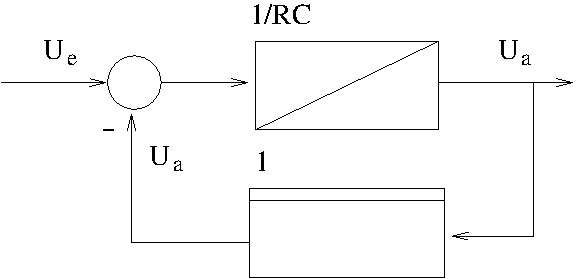
\includegraphics[width=7cm]{sysregel_bsb3}
\end{figure}
\begin{description}
\item[Man erkennt:] Es handelt sich hier ebenfalls um ein Verzögerungsglied 1. Ordnung. Unabhängig von der physikalischen Realisierung haben beide Systeme die gleiche dynamische Struktur!
\end{description}
\begin{bsp}[Erweiterung des Behälters um einen Schwimmer]
\end{bsp}
\begin{minipage}{.4\linewidth}
\begin{figure}[H]
  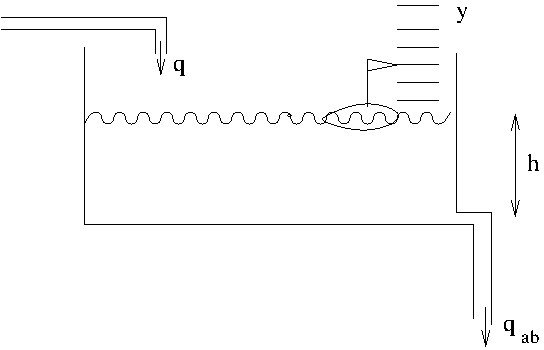
\includegraphics[height=4cm]{sysregel_bsp_4}
\end{figure}
\end{minipage}
\begin{minipage}{.6\linewidth}
\begin{align*}
\begin{array}{lll}
h&:& y $ in Ruhe$\\
m&:& $Masse des Schwimmers$\\
a&:& $Fläche des Schwimmers$\\
\rho&:& $Dichte der Flüssigkeit$\\
\end{array}
\end{align*}
\end{minipage}
Die Auftriebskraft ist gegeben durch $F= (h(t)-y(t))\cdot a \cdot \rho \cdot g$. Durch Umformen lässt sich hieraus die vom Zeiger des Schwimmers angezeigte Skalaposition berechnen:
\begin{equation*}
  F=m \cdot a = m \cdot \ddot{y}=(h(t)-y(t))\cdot a \cdot \rho \cdot g
\end{equation*}
\begin{equation*}
  \Leftrightarrow \ddot{y}= \frac{a \cdot \rho \cdot g}{m}(h(t)-y(t))
\end{equation*}
\begin{equation*}
  \Rightarrow y(t) = \frac{a \cdot \rho \cdot g}{m}\int_0^t{\int_0^\tau{h(T)-y(T)dT}d\tau}
\end{equation*}

\subsubsection*{BSB}

\begin{figure}[H]
  \centering
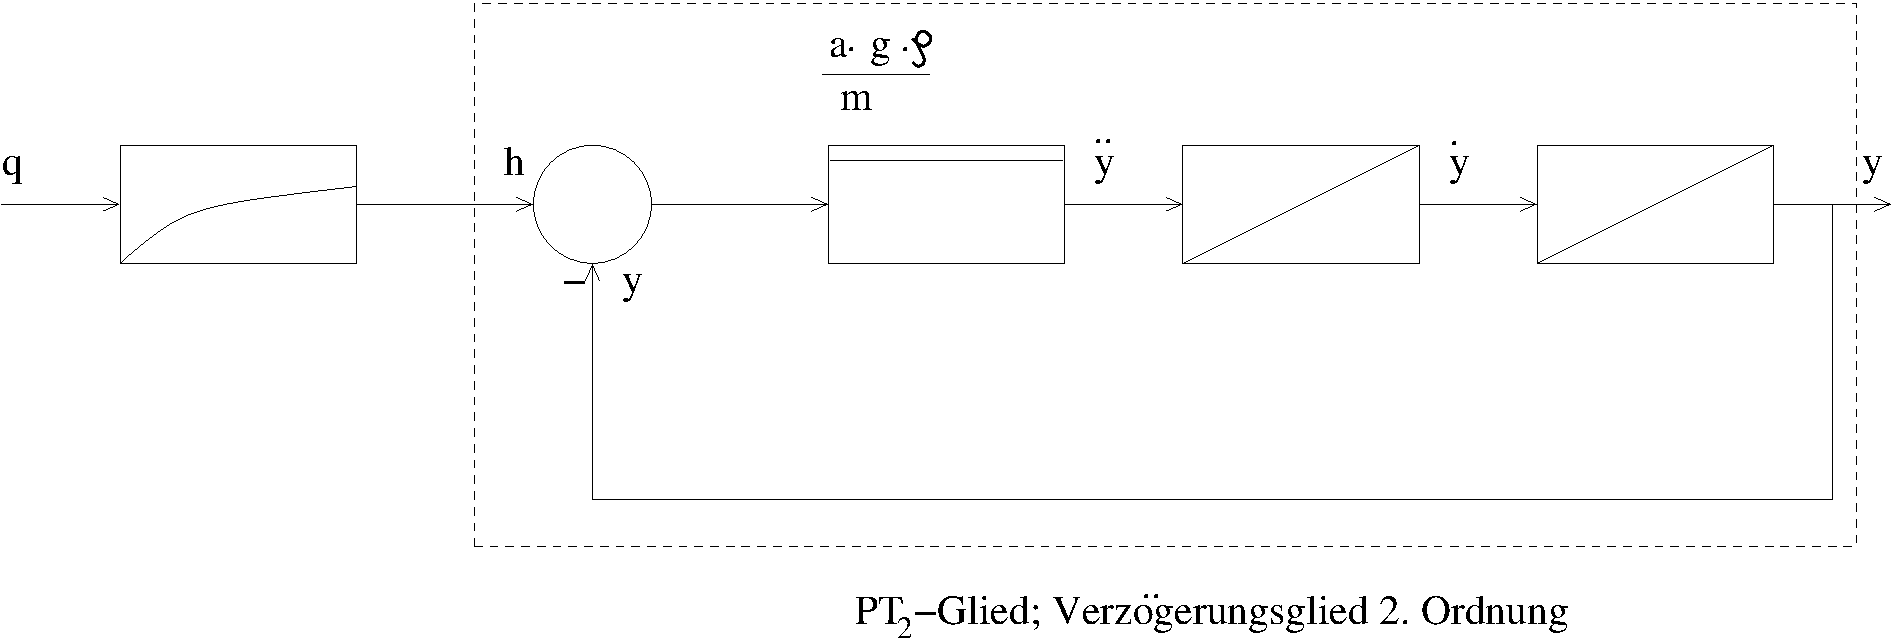
\includegraphics[width=.8\linewidth]{sysregel_bsb5}  
\end{figure}

Auch für das $PT_2$-Glied wird ein eigenes Standardsymbol definiert:
\begin{figure}[H]
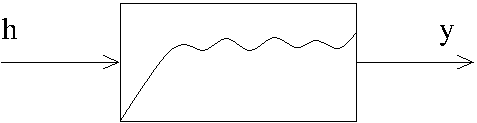
\includegraphics[width=5cm]{sysregel_pt2}
  
\end{figure}


\begin{bsp}[Zuleitung]
\end{bsp}
\begin{figure}[H]
\begin{minipage}{.6\linewidth}
\begin{figure}[H]
 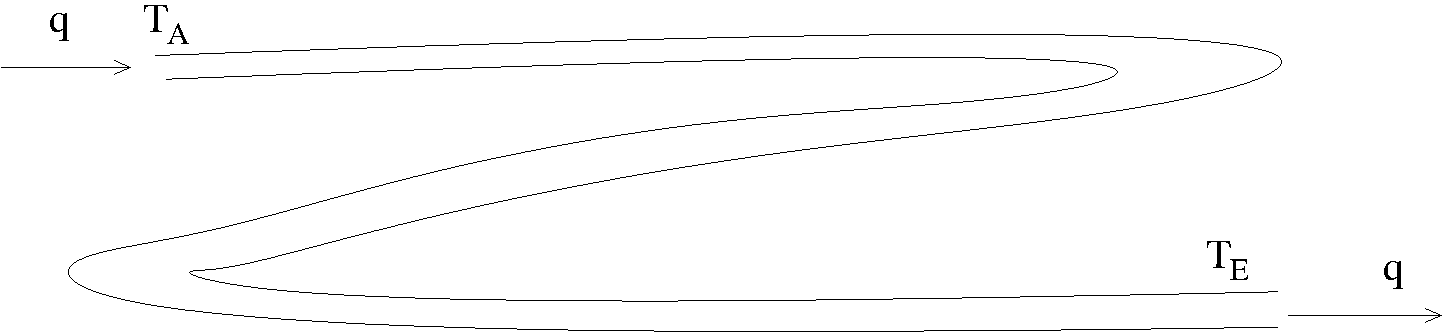
\includegraphics[width=.9\linewidth]{sysregel_bsp_5} 
\end{figure}
\end{minipage}
\begin{minipage}{.4\linewidth}
\begin{tabular}{lll}
$l$&:& Rohrlänge\\
$a$&:&Rohrquerschnitt\\
$v=\frac{q}{a}$&:& Fließgeschwindigkeit
\end{tabular}
\end{minipage}
\end{figure}

Die Zeit, bis eine Probemenge das Rohr durchflossen hat, wird \emph{Totzeit $T_t$} genennt. Sie ist gegeben durch
\begin{equation*}
  T_t=\frac{l}{v}=\frac{l \cdot a}{q}
\end{equation*}
$T_A$ und $T_E$ sind die Temperaturen am Rohranfang bzw. Rohrende. Unter der Annahme, dass das Rohr perfekt isoliert ist, beim Transport also keine Wärme verloren geht, hängen diese beiden Größen über die Sprungfunktion
\begin{equation*}
  T_E(t)=T_A(t-T_t)
\end{equation*}
zusammen. Dieser Zusammenhang wird im Blockschaubild durch das sogenannte \emph{Totzeitglied} dargestellt:
\begin{figure}[H]
  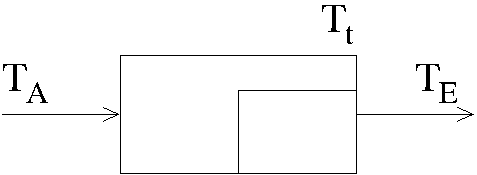
\includegraphics[width=4cm]{sysregel_tglied}
\end{figure}
\fancyhead{}
\fancyhead[LO,LE]{\leftmark}
\subsubsection*{Blockschaltbilder}
\begin{itemize}
\item beschreiben Ursache-Wirkungszusammenhänge in einer allgemeinen Form
\item sind insbesondere bei komplexen Systemen oft übersichtlicher als Darstellungen in Gleichungen
\item lassen sich schrittweise aufbauen und verifizieren
\item sind Basis für numerische Simulationen($\rightarrow$ Simulink)
\end{itemize}

\subsection{Häufig verwendete Übertragungsglieder}

\begin{itemize}
\item \textbf{elementare: }P,I,D,S,$T_t$
\item \textbf{zusammengesetzte: } $PT_1, PT_2$
\item \textbf{nichtlineare: } KL, M
\end{itemize}
In der Vorlesung werden hauptsächlich elementare und zusammengesetzte Übertragungsglieder verwendet!

\subsection{Nichtlineare Glieder und Linearisierung}

\begin{figure}[H]
  \begin{minipage}{.4\linewidth} %Anfang Bildbereich, 0,45 % der Seitenbreite
\begin{figure}[H]
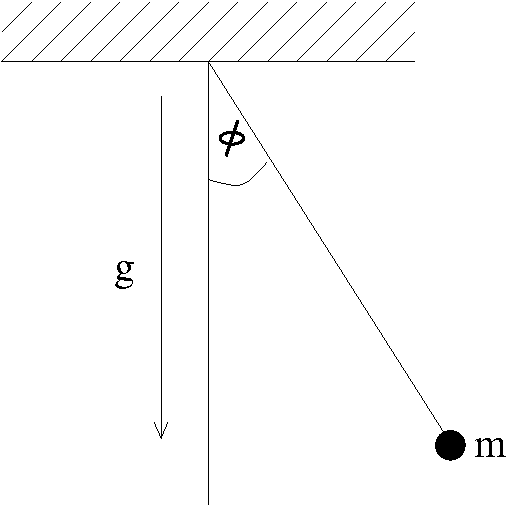
\includegraphics[height=5.5cm]{sysregel_bsp_6} % Hier Bild einfügen
\end{figure}
 \end{minipage}% Ende des Bildbereiches
  \begin{minipage}{.6\linewidth} %Anfang Formelbereich, 0,55 % der Seitenbreite
   \begin{align*}
    &&J*\ddot{\phi}&&=&&&M\\
\rightarrow&& m\cdot l^2 \cdot \ddot{\phi} &&=&&& -m\cdot g \cdot l \cdot sin(\phi)\\
\rightarrow&& l \cdot \ddot{\phi}&&=&&&-g*sin(\phi)\\
\rightarrow&& \ddot{\phi}&&=&&& -\frac{g}{l}sin(\phi)
   \end{align*}
   \begin{tabular}{lll}
$J$&:& Trägheitsmoment\\
$M$&:& Drehmoment
  
   \end{tabular}

\end{minipage}% Ende des Tabellenbereiches
\end{figure}

Erneut wird das Blockschaltbild aufgestellt, unter Verwendung des sog. \emph{Kennliniengliedes} (KL-Glied):

\begin{figure}[H]
  \centering
  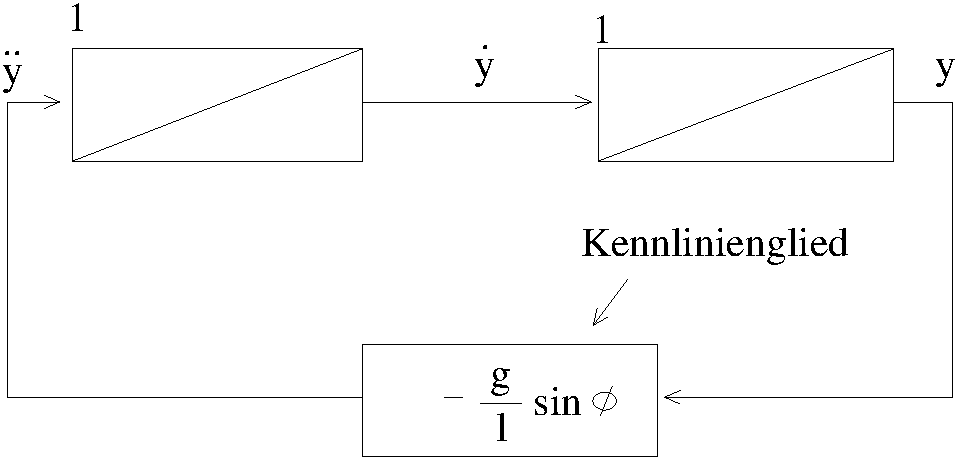
\includegraphics[width=.5\linewidth]{sysregel_bsb4}
\end{figure}

Ein nichtlineares System lässt sich zwar numerisch simulieren, stellt aber ein Problem bei der Analyse oder beim Regelentwurf dar. Als Hilfsmittel wird daher eine Linearisierung im Arbeitspunkt verwendet.
\begin{description}
\item[Arbeitspunkt: ]Betriebszustand eines Systems, in dem die zeitveränderlichen Größen fest sind (stationärer Zustand) und sich das System in einem gewünschten Sollzustand befindet. 
\end{description}
Wird das System nun um den Arbeitspunkt linearisiert, sind die Abweichungen zwischen nichtlinearem und linearem Modell \emph{in der Umgebung um diesen Arbeitspunkt herum }nur klein. Bei zu großer Abweichung vom Arbeitspunkt bildet das lineare Modell das nichtlineare nur unzureichend ab. Der Arbeitspunkt muss dann verändert/neu bestimmt werden. 

\subsubsection*{Linearisierung eines KL-Gliedes}
\begin{figure}[H]
\center
  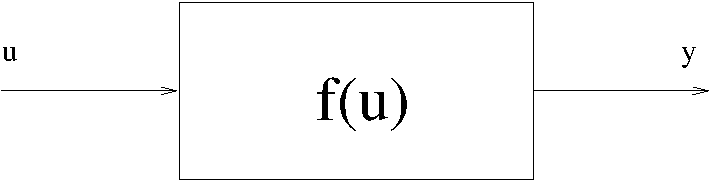
\includegraphics[width=6cm]{sysregel_klglied}
\end{figure}

\begin{eqnarray*}
  y&=&f(u) \\
y_0+ \Delta y &=& f(u_0+ \Delta u)
\end{eqnarray*}
Es wird nun die Taylorreihen-Entwicklung für diese Funktion durchgeführt:
\begin{eqnarray*}
  y_0+\Delta y &=& f(u_0) + [\frac{df(u)}{du}]_{u_0} \cdot \Delta u + \dots\\
  \Rightarrow y_0& =& f(u_0)\\ \Delta y &=&[\frac{df(u)}{du}]_{u_0} \cdot \Delta u + \dots \text{ (Nichtlineare Terme werden Vernachlässigt!)}
\end{eqnarray*}
z.B. $y=sin(\phi)$: Linearisierung um den Arbeitspunkt $\phi_0 =0$
\begin{eqnarray*}
y_0 &=& 0\\
\Delta y&=& [cos(\phi)]_{\phi_0 =0} \cdot \Delta \phi\\
\Rightarrow T_y &=& 1 \cdot \Delta \phi 
\end{eqnarray*}

\begin{figure}[H]
\center
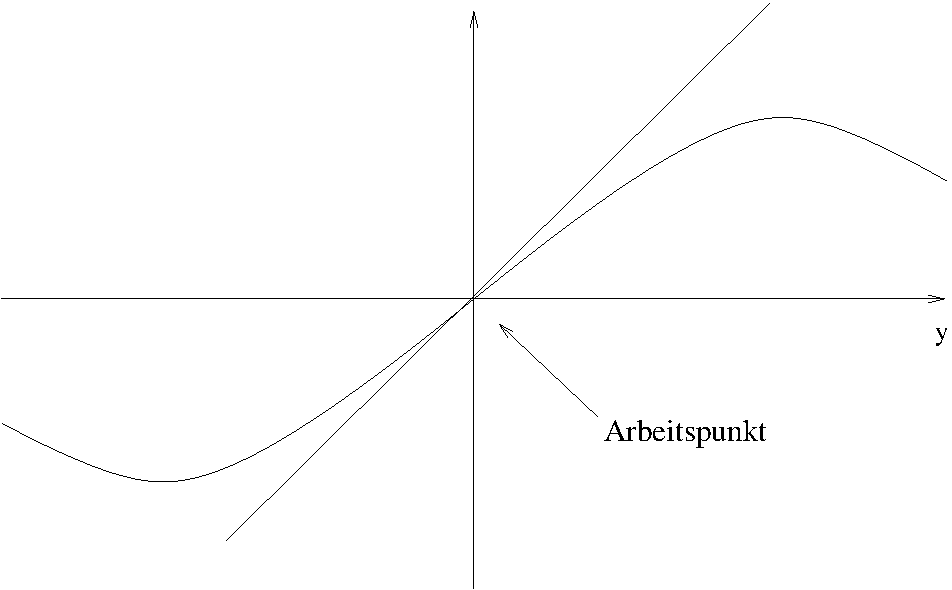
\includegraphics[width=8cm]{sysregel_linear}
\end{figure}

\section{Systembeschreibung im Zeitbereich}

\subsection{Differentialgleichungen}

\subsubsection{Aufstellen der DGL}

Die Differentialgleichung eines Systems kann auf 2 Arten bestimmt werden:
\begin{itemize}
\item aus den physikalischen Gleichungen, z.B.:
  \begin{itemize}
  \item Bewegungsgleichungen: $F(t)=m \cdot \ddot{x}(t)$ ; $M(t)=J \cdot \ddot{\phi}$
  \item Bilanzierung von Volumen: $q_{zu}(t)-q_{ab}(t)=\dot{v}(t)$ 
  \end{itemize}
\item aus dem Blockschaubild:
  \begin{itemize}
  \item eventuell Hilfsgrößen einführen (z.B. Ausgang von S-Gliedern,\dots
  \item Entgegen der Signalflussrichtung durch das BSB gehen und Funktionsbeziehungen der Blöcke auswerten
   \end{itemize}
\end{itemize}
\textbf{Bsp.:} $PT_1$-Glied

   \begin{figure}[H]
     \centering
     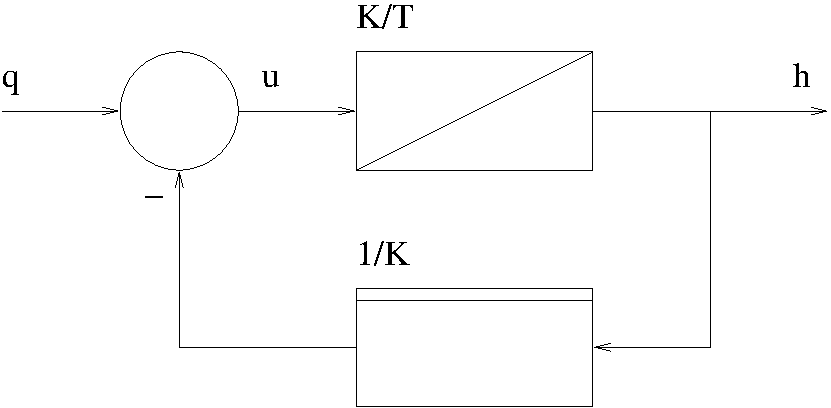
\includegraphics[width=.5\linewidth]{sysregel_bsb6}
   \end{figure}
   \begin{math}
     \begin{array}{llll}
       &h(t)&=&\frac{K}{T}\int_0^t{u(\tau)d\tau}\\
     \rightarrow&\dot{h}(t)&=&\frac{K}{T}\cdot u(t)\\
     &u(t)&=&q-\frac{1}{K}\cdot h(t)\\
     \Rightarrow&\dot{h}(t)&=&\frac{K}{T}\cdot (q(t)-\frac{1}{K} \cdot{h}(t))\\
     \Rightarrow&\frac{1}{T}\cdot h(t)+\dot{h}(t)&=&\frac{K}{T}\cdot q(t)\\
     \Rightarrow&\underbrace{h(t)+T\cdot \dot{h}(t)}_{\text{DGL in }h(t)}&=&\underbrace{k\cdot q(t)}_{\text{Anregung}}\\

     \rightarrow& \multicolumn{3}{l}{\text{homogene DGL, falls }q(t)=0 \text{ (Anregung}=0)}
   \end{array}
  \end{math}

  \subsubsection{Lösung von Differentialgleichungen mit konstanten Koeffizienten}

  \begin{bsp}[Lösung der DGL des $PT_1$-Gliedes]
\end{bsp}
Gegeben ist die Gleichung
\begin{equation*}
  T\cdot \dot{y}(t)+y(t)=k\cdot u(t)
\end{equation*}
mit $y(0)=y_0$ und beliebigem $u(t)$ für $t>0$.
\begin{itemize}
\item \textbf{1. Schritt:} characteristische Gleichung:\\
  \begin{math}
    \begin{array}{llllllll}
      &T\cdot s +1&=&0\\
      \rightarrow&s_1&=&-\frac{1}{T}\\
      \Rightarrow&y_h(t)&=&C_1\cdot y_1(t)&=&c_1*e^{-\frac{t}{T}}&\text{(Formelsammlung)}
    \end{array}
  \end{math}
\item \textbf{2. Schritt:} Variation der Konstanten\\
  \begin{math}
    \begin{array}{lllllllll}
                       &y_p(t)&=&C_1(t)e^{-\frac{t}{T}}\\
      \text{ableiten: }&\dot{y_p}(t)&=&\frac{-C_1(t)}{T}e^{-\frac{t}{T}}+\dot{C_1}(t)e^{-\frac{t}{T}}\\
\multicolumn{4}{l}{\text{In die inhomogene DGL einsetzen:}}\\
&K\cdot u(t)&=&T\cdot (-\frac{\cancel{c_1(t)}}{T}\cdot \cancel{e^{-\frac{t}{T}}}+\dot{C_1}(t)\cdot e^{-\frac{t}{T}})+\cancel{C_1(t)\cdot e^{-\frac{t}{T}}}\\
&\dot{C_1}(t)&=&\frac{K}{T}\cdot e^{\frac{t}{T}}\cdot u(t)\\
\text{Integrieren:}&C_1(t)&=&\int_0^t{\frac{K}{T}\cdot e^{\frac{\tau}{T}}\cdot u(\tau)d\tau}\\
\Rightarrow&y_p(t)&=&[\int_0^t{\frac{K}{T}\cdot e^{\frac{\tau}{T}}\cdot u(\tau)d\tau}]\cdot e^{-\frac{t}{T}}\\
&&=&\int_0^t{\frac{K}{T}\cdot e^{-\frac{t-\tau}{T}}\cdot u(\tau)d\tau}

    \end{array}
  \end{math}
\item \textbf{3. Schritt:} Zusammenfassen zur Gesamtlösung\\
  \begin{math}
    \begin{array}{lll}
      y(t)&=&y_n(t)+y_p(t)\\
          &=&c_1\cdot e^{-\frac{t}{T}}+\int_0^t{\frac{K}{T}\cdot e^{-\frac{t-\tau}{T}}\cdot u(\tau)d\tau}
    \end{array}
  \end{math}
\item \textbf{4. Schritt:} $C_1$ bestimmen\\
  \begin{math}
    \begin{array}{llll}
     &y(0)&=&C_1=y_0\\
     \Rightarrow \text{Lösung:}&y(t)&=&\underbrace{y_0\cdot e^{-\frac{t}{T}}}_{1}+\underbrace{\int_0^t{\frac{K}{T}\cdot e^{-\frac{t-\tau}{T}}\cdot u(\tau)d\tau}}_{2}
    \end{array}
  \end{math}
  \begin{itemize}
  \item \textbf{Formelteil 1} ist die homogene Lösung. Sie ist nur vom Anfangswert $y_0$ abhängig. Man sagt: Sie beschreibt die \emph{freie Bewegung}
  \item \textbf{Formelteil 2} ist die Partikulärlösung. Sie ist nur von der Eingangsfunktion $u(t)$ abhängig. Man sagt: Sie beschreibt die \emph{erzwungene Bewegung}
  \end{itemize}
\end{itemize}

\subsection{Übertragungsverhalten}

\subsubsection{Gewichtsfunktion und Faltung}

Das Übertragungsverhalten von $u(t)$ zu $y(t)$ wird durch den Term
\begin{equation*}
  y(t)=\int\limits_0^t{\frac{K}{T}\cdot e^{\frac{-t-\tau}{T}}\cdot u(\tau)d\tau}
\end{equation*}
definiert. Er beschreibt das Übertragungsverhalten bei verschwindenden Anfangsbedingungen ($y_0=0$). Mit der Funktion
\begin{equation*}
  g(t)=\frac{K}{T}\cdot e^{-\frac{t}{T}}
\end{equation*}
lässt sich das Integral zu
\begin{equation*}
  y(t)=\underbrace{\int\limits_0^t{g(t-\tau)\cdot u(\tau)d\tau}}_{Faltungsintegral}=g(t)*u(t)
\end{equation*}
vereinfachen. Das Zeichen $*$ wird als ``gefaltet mit'' ($g(t)$ gefaltet mit $u(t)$) gelesen. \\
$g(t)$ nennt man \emph{Gewichtsfunktion}. Sie beschreibt das Übertragungsverhalten des Systems vollständig!

\begin{description}
\item[Es gilt:] $g(t)*u(t)=u(t)*g(t)$
\end{description}
Die Gewichtsfunktion $g(t)$ gibt an, mit welchem Gewicht der Wert der Eingangsfunktion $u(t)$ von \emph{zurückliegenden} Zeitpunkten $(t-\tau)$ in den Wert der Ausgangsfunktion $y(t)$ zum \emph{aktuellen} Zeitpunkt $t$ eingeht.\\
\begin{figure}[H]
  \centering
  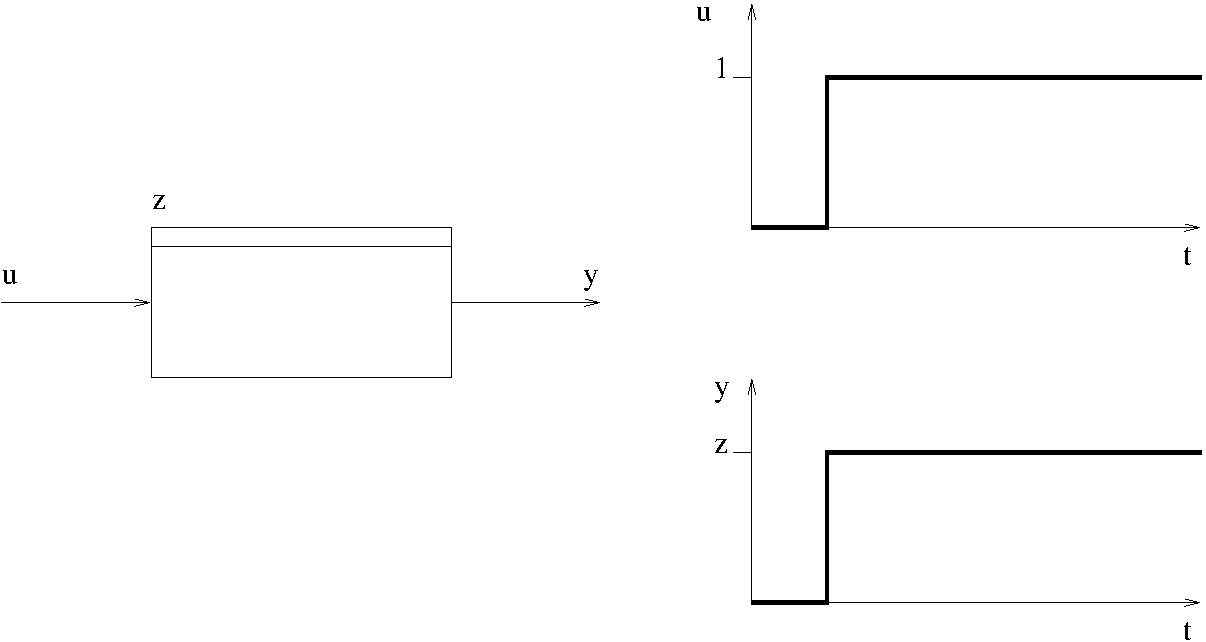
\includegraphics[height=5cm]{sysregel_gewfkt_1}
\end{figure}
Der Ausgang hängt nur vom aktuellen Eingang ab.
\begin{figure}[H]
  \centering
  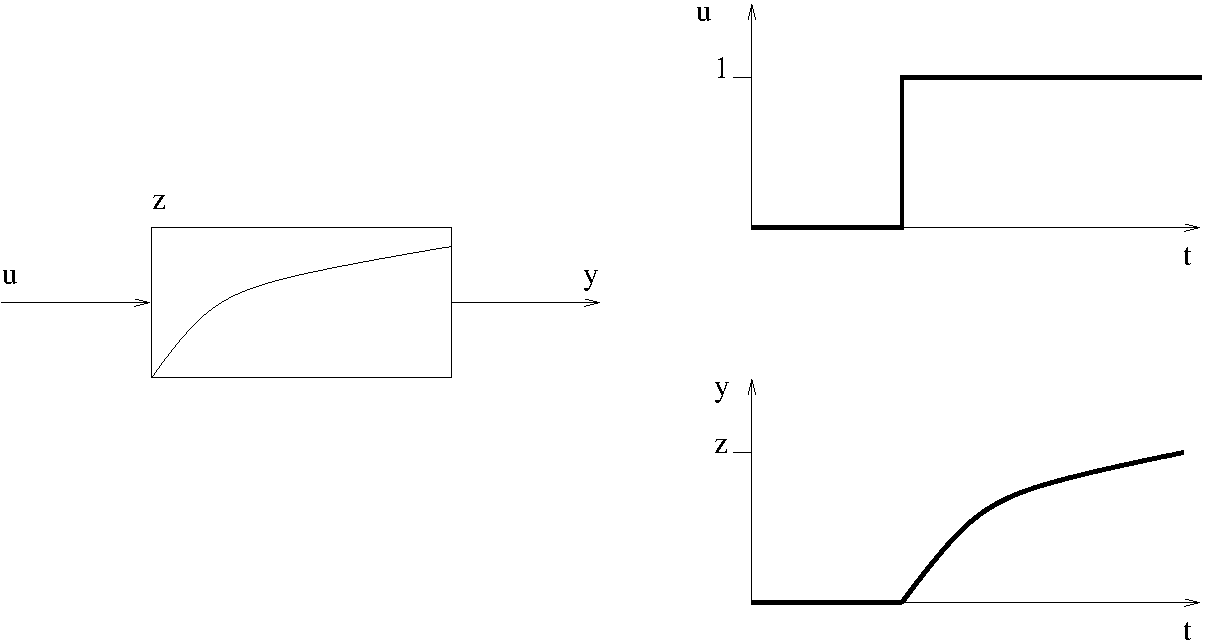
\includegraphics[height=5cm]{sysregel_gewfkt_2}
\end{figure}
In diesem Fall hingegen ist der Ausgang auch von vergangenen Werten abhängig.
\subsubsection{Eigenschaften}
\textbf{Lineare} und \textbf{zeitinvariante} Systeme lassen sich durch die Gewichtsfunktion vollständig beschreiben. (Entspricht der linearen DGL mit konstanten Koeffizienten)
\begin{description}
\item[Linearität:] Ein System ist linear, wenn...
  \begin{itemize}
  \item ...das Superpositionsprinzip: $y(t)=g(t)*[u_1(t)+u_2(t)]=g(t)*u_1(t)+ g(t)*u_2(t)$
  \item ...das Verstärkungsprinzip: $y(t)=g(t)*[\alpha \cdot u(t)]= \alpha \cdot[g(t)*u(t)]$
  \end{itemize}
gelten.
\item[Zeitinvarianz:] Das System ist invariant gegenüber Zeitverschiebungen: \\
Aus $y(t)=g(t)*u(t)$ muss für eine beliebige Zeitverschiebung $T$ folgen, dass $y(t-T)=g(t)*u(t-T)$
\item[Kausalität:] Das Ausgang $y(t)$ eines kausalen Systems hängt \emph{nur} vom Verlauf des Eingangs $u(t)$ für Zeiten $t\le t_0$ ab. Das System hängt also nur von vergangenen Eingangswerten ab. Für $g(t)$ kausaler Systeme gilt also:
  \begin{equation*}
    g(t)=0 \text{ für } t<0
  \end{equation*}
\end{description}

\subsubsection{Sprungsantwort und Impulsantwort}

\begin{description}
\item[Sprungantwort:] Auf den Systemeingang wird ein \emph{Einheitssprung} gegeben

  \begin{figure}[H]
    \centering
    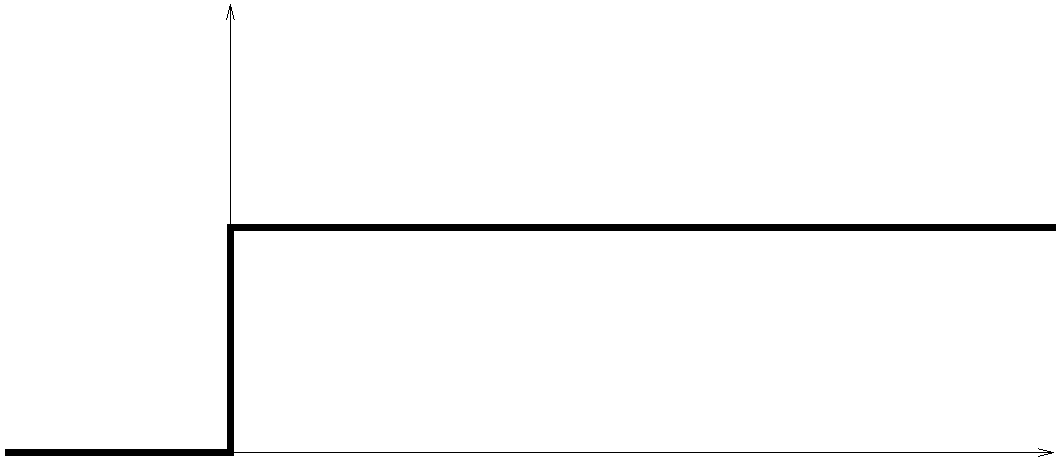
\includegraphics[width=6cm]{sysregel_einheitssprung}
  \end{figure}
  \begin{equation*}
    u(t)=\sigma (t) =\begin{cases} 0 $ für $t<0\\1 $ für $ t \geq 0\end{cases}
  \end{equation*}
Die Antwort des Systems heißt \emph{Sprungantwort} und wird beschrieben durch
\begin{equation*}
  h(t):=y(t)
\end{equation*}
Mit dem Flächenintegral $y(t)=\int\limits_0^t{g(\tau)\cdot u(t-\tau)d\tau}$ vereinfacht sich das zu
\begin{align*}
  \begin{array}{lll}
    h(t)&=&\int\limits_0^t{g(\tau)\cdot \underbrace{\sigma (t-\tau)}_{=1}d\tau}\\
    h(t)&=&\int\limits_0^t{g(\tau)d\tau}  
  \end{array}
\end{align*}
Die Sprungantwort, genau wie die Gewichtsfunktion, characterisiert das dynamische System vollständig!
\item[Impulsantwort: ] Die Impulsfunktion $\delta (t)$ ist die formale Ableitung des Einheitssprungs.
  \begin{equation*}
    \delta (t)=\frac{d}{dt}\sigma (t) \Leftrightarrow \int\limits_0^t{\delta(\tau)d\tau =\sigma(t)}
  \end{equation*}
Für die Impulsantwort gilt damit:
\begin{equation*}
  \int\limits_0^t{g(\tau)\cdot u(t-\tau)d\tau} =\int\limits_0^t{g(\tau)\cdot \delta(t-\tau)d\tau }=g(t)
\end{equation*}
$\Rightarrow$ Die Gewichtsfunktion $g(t)$ kann auch als Impulsantwort interpretiert werden.

\end{description}

\subsection{Darstellung im Zustandsraum}

\begin{figure}[H]
\begin{bsp}[System aus 3 verbundenen Wassertanks]
\end{bsp}
  \centering
  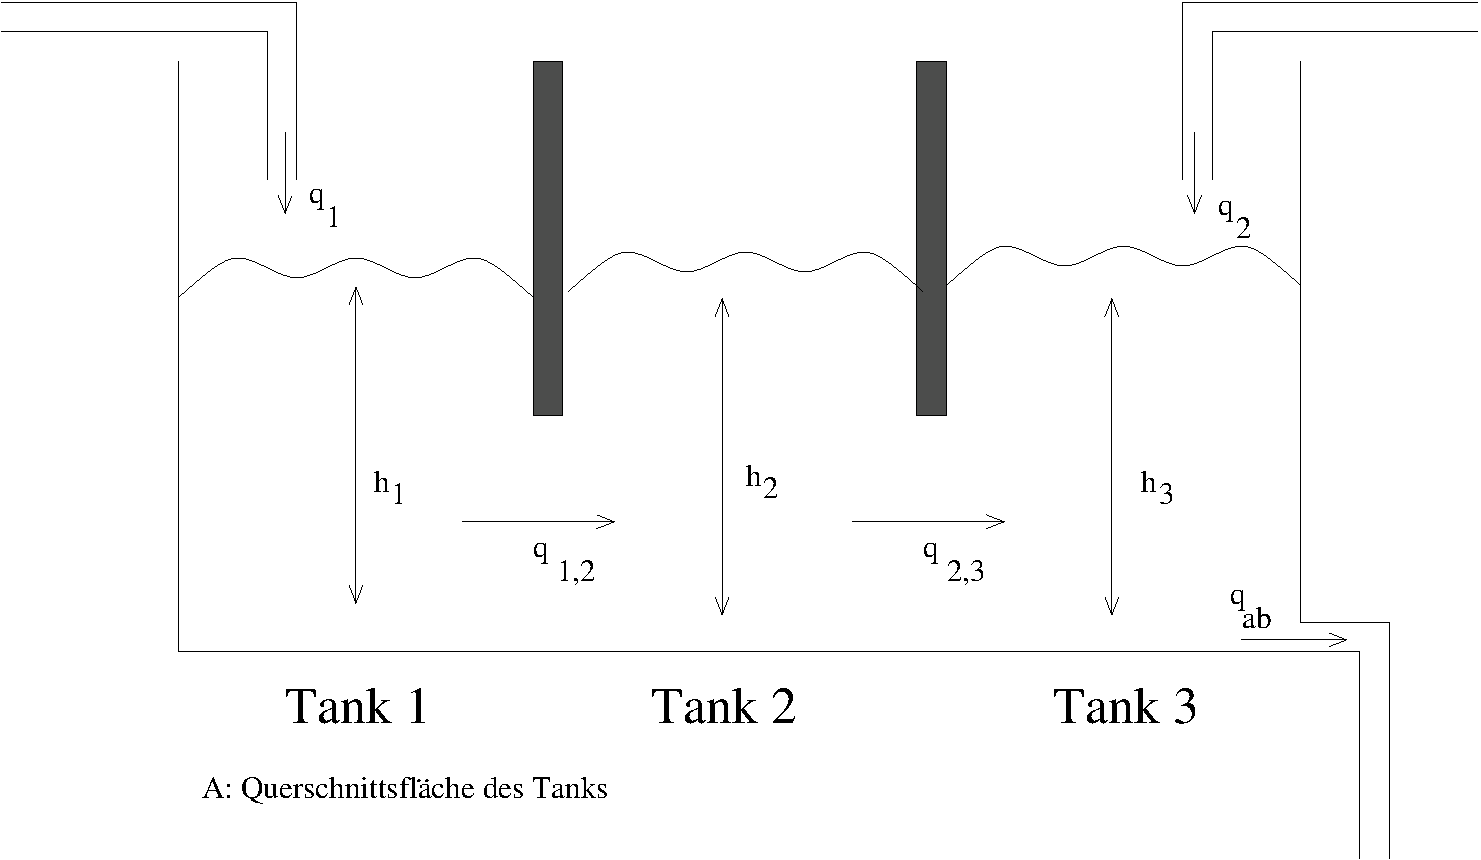
\includegraphics[width=.9\linewidth]{sysregel_bsp_2,2}
\end{figure}
Volumenbilanz:
\begin{align*}
  \begin{array}{llll}
    \text{Tank 1:}&\dot{h_1}&=&\frac{1}{A}(q_1-q_{1,2})\\
    \text{Tank 2:}&\dot{h_2}&=&\frac{1}{A}(q_{1,2}-q_{2,3})\\
    \text{Tank 3:}&\dot{h_3}&=&\frac{1}{A}(q_{2}+q_{2,3}-q_{ab})
  \end{array}
\end{align*}
\begin{description}
\item[Annahme:]Der Ausgleichsfluss zwischen den Tanks ist proportional zur Füllstandsdifferenz: \begin{center}  $q_{1,2}=c\cdot (h_1-h_2);q_{2,3}=c\cdot (h_2-h_3);q_{ab}=ch_3$ \end{center}
\end{description}
\begin{align*}
  \begin{array}{llll}
    \text{damit:}&\dot{h_1}&=&\frac{1}{A}(q_1-ch_1+ch_3)\\
                 &\dot{h_2}&=&\frac{1}{A}(ch_1-2ch_2+ch_3)\\
                 &\dot{h_3}&=&\frac{1}{A}(q_2+ch_2-2ch_3)
  \end{array}
\end{align*}
Kennt man $h_1,h_2,h_3$, so ist der Zustand des Systems zum Zeitpunkt t vollständig bestimmt. $\Rightarrow h_1,h_2,h_3$ sind die Zustandsgrößen des Systems.\\
\textbf{Geometrische Deutung:} $h_1,h_2,h_3$ spannen einen dreidimensionalen Vektorraum auf, den sogenannten \emph{Zustandsraum}.\\
\begin{figure}[H]
  \begin{minipage}{0.5\linewidth}
    \begin{figure}[H]
      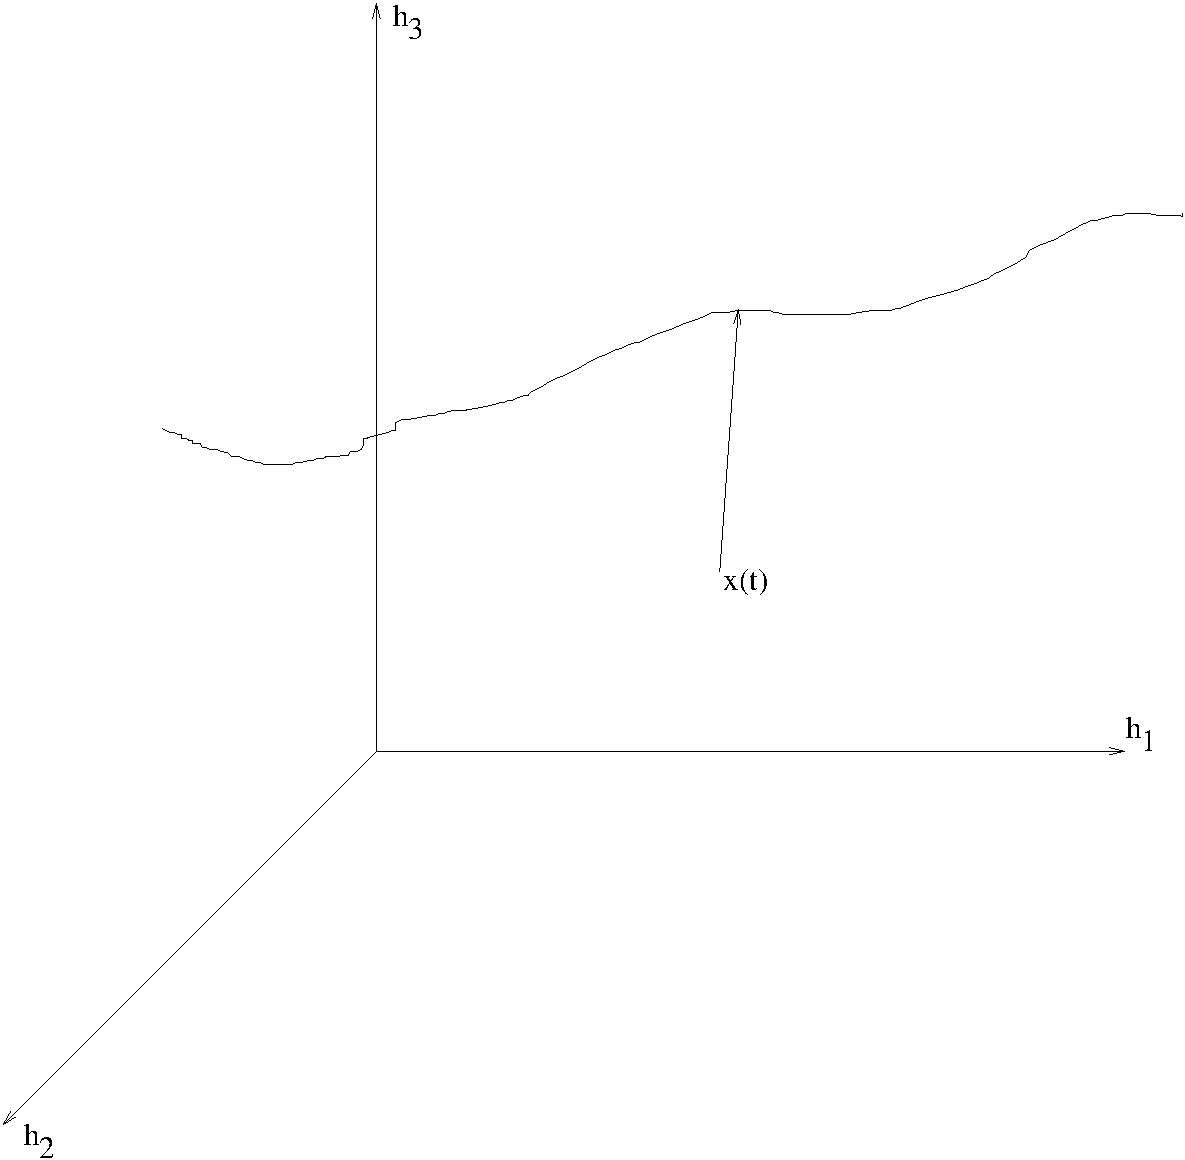
\includegraphics[width=0.9\linewidth]{sysregel_zustandsraum}
    \end{figure}
  \end{minipage}
  \begin{minipage}{0.5\linewidth}
    \[\vec{x}(t): \text{Zustandsvektor}\\\]
    \[\vec{x}(t)=  \begin{pmatrix}
            h_1(t) \\
            h_2(t) \\
            h_3(t) \end{pmatrix} \] 
  \end{minipage}
\end{figure}
Das System wird durch $q_1(t)$ und $q_2(t)$ angeregt, diese sind die \emph{Eingangsgrößen}. Aus ihnen lässt sich der sogenannte \emph{Eingangsvektor} bestimmen:
\begin{equation*}
  \vec{u}(t)=\begin{pmatrix}
                            q_1(t)\\
                            q_2(t)
             \end{pmatrix}
\end{equation*}

\subsubsection*{Verallgemeinerung}

Das Systrem lässt sich durch $n$ Zustände beschreiben:
\[
\vec{x}=
\begin{pmatrix}
x_1\\
x_2\\
\vdots\\
x_n
\end{pmatrix}
\]
Das Systrem besitzt $m$ Eingänge:
\[
\vec{u}=
\begin{pmatrix}
u_1\\
u_2\\
\vdots\\
u_m
\end{pmatrix}
\]
Dieses System lässt sich durch $n$ DGL 1 Ordnung beschreiben:
\[
\left.
\begin{array}{cc}
x_1=f_1(\vec{x},\vec{u})\\
\vdots\\
x_n=f_n(\vec{x},\vec{u})
\end{array}
\right\}
\begin{array}{ll}
\vec{x}(t)=\vec{f}(\vec{x}(t),\vec{u}(t))\\
\text{Zustandsdifferentialgleichung}
\end{array}
\]
Durch Messung des Systems wird aus dem aktuellen Zustand $\vec{x}(t)$ und dem Eingang $\vec{u}(t)$ der Ausgangsvektor $\vec{y}(t)$ bestimmt. Die daraus resultierende Gleichung
\begin{equation*}
  \vec{y}(t)=g(\vec{x}(t),\vec{u}(t))
\end{equation*}
heißt \emph{Ausgangsgleichung}. $\vec{y}(t)$ ist gegeben durch 
\begin{equation*}
  \vec{y}(t)=
\begin{pmatrix}
y_1\\
\vdots\\
y_p
\end{pmatrix}
\end{equation*}
Da man bei komplexen Systemen mit mehreren Ein- und Ausgängen für jedes Eingang/Ausgangpaar eine eigene Gewichtsfunktion aufstellen müsste, bietet sich bei der Simulation solcher Systeme die Zustandsraumdarstellung an.\\  
Die Beschreibung eines Systems im Zustandsraum oder allgemein durch Gleichungen ist der Darstellung im Blockschaubild äquivalent. Je nach Anwendung wird die optimale Beschreibung gewählt. 
%Mindmap ab hier!
\begin{figure}[H]
\centering
                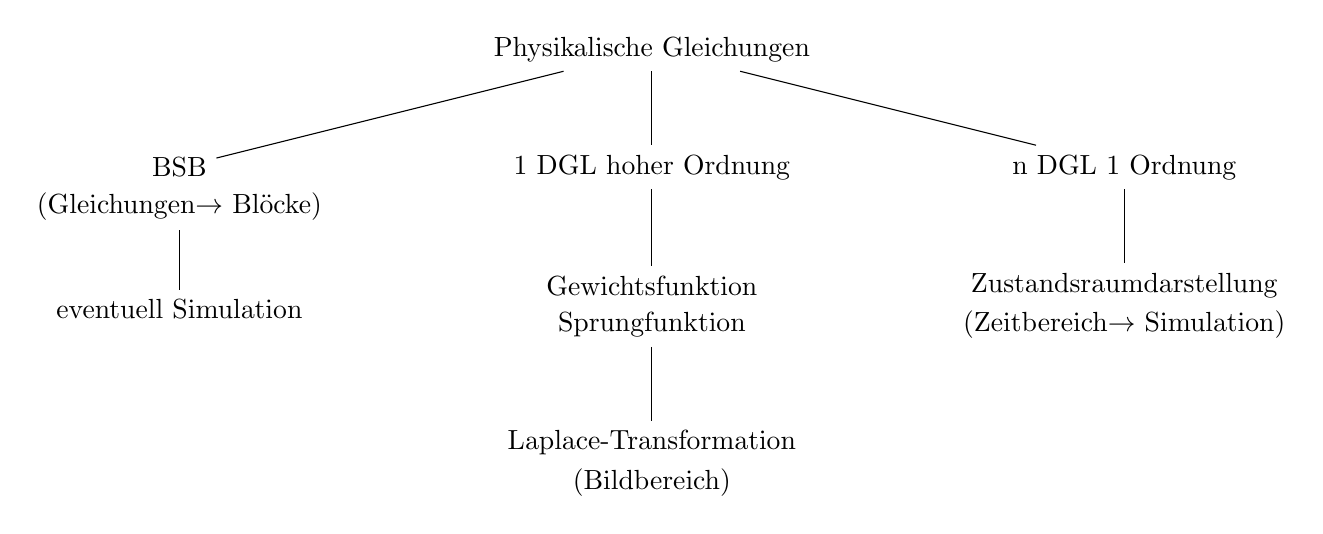
\begin{tikzpicture}
                  \node {Physikalische Gleichungen}
                    child[sibling distance=6cm] {node {BSB}
                     child[level distance=0.5cm]{node {(Gleichungen$\rightarrow$ Blöcke)}edge from parent[draw=none]
                      child[level distance=1.3cm]{node {eventuell Simulation}}
                     }
                  }       
                    child[sibling distance=6cm] {node {1 DGL hoher Ordnung}
                      child {node {Gewichtsfunktion}
                        child[level distance=0.5cm]{node {Sprungfunktion}edge from parent[draw=none]
                         child[level distance=1.5cm]{node{Laplace-Transformation}
                           child[level distance=0.5cm]{node {(Bildbereich)}edge from parent[draw=none]}
}
}
}
}
                    child[sibling distance=6cm] {node {n DGL 1 Ordnung}
                      child {node {Zustandsraumdarstellung}
                         child[level distance=0.5cm]{node {(Zeitbereich$\rightarrow$ Simulation)}edge from parent[draw=none]
                        }
}
                          };
                \end{tikzpicture}
\end{figure}

\subsubsection{Numerische Simulation}

\textbf{gegeben:}
\begin{align*}
  \vec{\dot{x}}(t)=\vec{f}(\vec{x}(t),\vec{u}(t))(*)\\
  \text{Anfangswert } \vec{x}(0)=\vec{x_0}\\
\end{align*}
\textbf{gesucht:} numerische Näherung ${\tilde{x}}$ für die Lösung der DGL auf einem Zeitintervall $[0,t_{max}]$\\
\textbf{Idee: } Approximation von $\vec{\dot{x}}(t)$ durch den Differenzenquotienten:
\begin{equation*}
  \vec{\dot{x}}\approx \frac{\vec{x}(t+h)-\vec{x}(t)}{h} \text{ mit Zeitschritt }h
\end{equation*}
\textbf{Einsetzen in $(*):$ }
\begin{align*}
  \begin{array}{lll}
   \frac{\vec{x}(t+h)-\vec{x}(t)}{h} &\approx& \vec{f}(\vec{x}(t),\vec{u}(t)) \\
   \Rightarrow \vec{x}(t)+h \cdot \vec{f}(\vec{x}(t),\vec{u}(t)) &\approx&x(t+h)
   \end{array}
\end{align*}
mit festen Zeitschritten $t_i=i\cdot h$
\begin{equation*}
  \underbrace{\vec{\tilde{x}}(t_{i+1})}_{\text{neuer Zustand}}=\underbrace{\vec{\tilde{x}}(t_i)}_{\text{alter Zustand}}+h \cdot \vec{f}(\vec{x}(t_i),\vec{u}(t_i))
\end{equation*}
Diese Gleichung lässt sich mithilfe des \emph{Euler-Verfahrens} lösen.

\subsubsection{Lineare Systeme}

\textbf{Fortsetzung Bsp 2.2:}\\
Sortieren der Zustände und der Eingänge:
\begin{align*}
  \begin{array}{lllllllllllll}
    \dot{h_1}(t)&=&-&\frac{C}{A}h_1(t)&+&\frac{C}{A}h_2(t)&&&+&\frac{1}{A}q_1(t)\\
    \dot{h_2}(t)&=&&\frac{C}{A}h_1(t)&-&\frac{2C}{A}h_2(t)&+&\frac{C}{A}h_3(t)\\
    \dot{h_3}(t)&=&&&&\frac{C}{A}h_2(t)&-&\frac{2C}{A}h_3(t)&&&+&\frac{1}{A}q_2(t)
  \end{array}
\end{align*}
Die obige Gleichung lässt sich auch in Vektoren und Matrizen ausdrücken:
\begin{align*}\underbrace{
  \begin{pmatrix}
    \dot{h_1}\\
    \dot{h_2}\\
    \dot{h_3}
  \end{pmatrix}}_{\vec{\dot{x}}(t)}
=
\underbrace{
\begin{pmatrix}
  -\frac{C}{A}&+\frac{C}{A}&0\\
  \frac{C}{A}&-\frac{2C}{A}&\frac{C}{A}\\
  0&\frac{C}{A}&-\frac{2C}{A}
\end{pmatrix}}_{\text{Systemmatrix }\mathbf{A}}
\cdot
\underbrace{
\begin{pmatrix}
h_1(t)\\
h_2(t)\\
h_3(t)  
\end{pmatrix}}_{\parbox{1cm}{\scriptsize Zustands\-vektor~$\vec{x}(t)$}}
+
\underbrace{
\begin{pmatrix}
\frac{1}{A}&0\\
0&0\\
0&\frac{1}{A}  
\end{pmatrix}}_{\parbox{1cm}{\scriptsize Eingangs\-matrix~$\mathbf{B}$}}
\cdot
\underbrace{
  \begin{pmatrix}
    q_1(t)\\
    q_2(t)\\
~
  \end{pmatrix}}_{\parbox{1cm}{\scriptsize Eingangsvektor~$\vec{u}$}}
\end{align*}
Diese Gleichung gilt nur bei linearen Systemen und ist außerdem eine beliebte \textbf{Klausuraufgabe!} Allgemein gilt:
\begin{align*}
  \begin{array}{lllllll}
    \vec{x}(t)&=&\mathbf{A}\cdot\vec{x}(t)&+&\mathbf{B}\cdot\vec{u}(t)&\text{Zustandsdifferentialgleichung}\\
    y(t)&=&\mathbf{C}\cdot \vec{x}(t)&+&\mathbf{B}\cdot\vec{u}(t)&\text{Ausgangsgleichung}
  \end{array}
\end{align*}

\subsubsection{Aufstellen der Zustandsgleichung aus BSB und DGL}

\paragraph{aus dem Blockschaubild}
\begin{description}
\item[Idee:] Jedes I-Glied (und $PT_1$) speichert einen Zustand. Um die Zustandsgleichung aufzustellen muss also wie folgt vorgegangen werden:
  \begin{enumerate}
  \item $PT_2$-Glieder zerlegen
  \item Alle Ausgänge von I- und $PT_1$-Gliedern als Zustände einführen (Buchstaben im BSB zuweisen!)
  \item Entgegen der Signalflussrichtung die Gleichungen bestimmen
  \end{enumerate}
\end{description}
\begin{figure}[H]
\begin{bsp}
\end{bsp}
  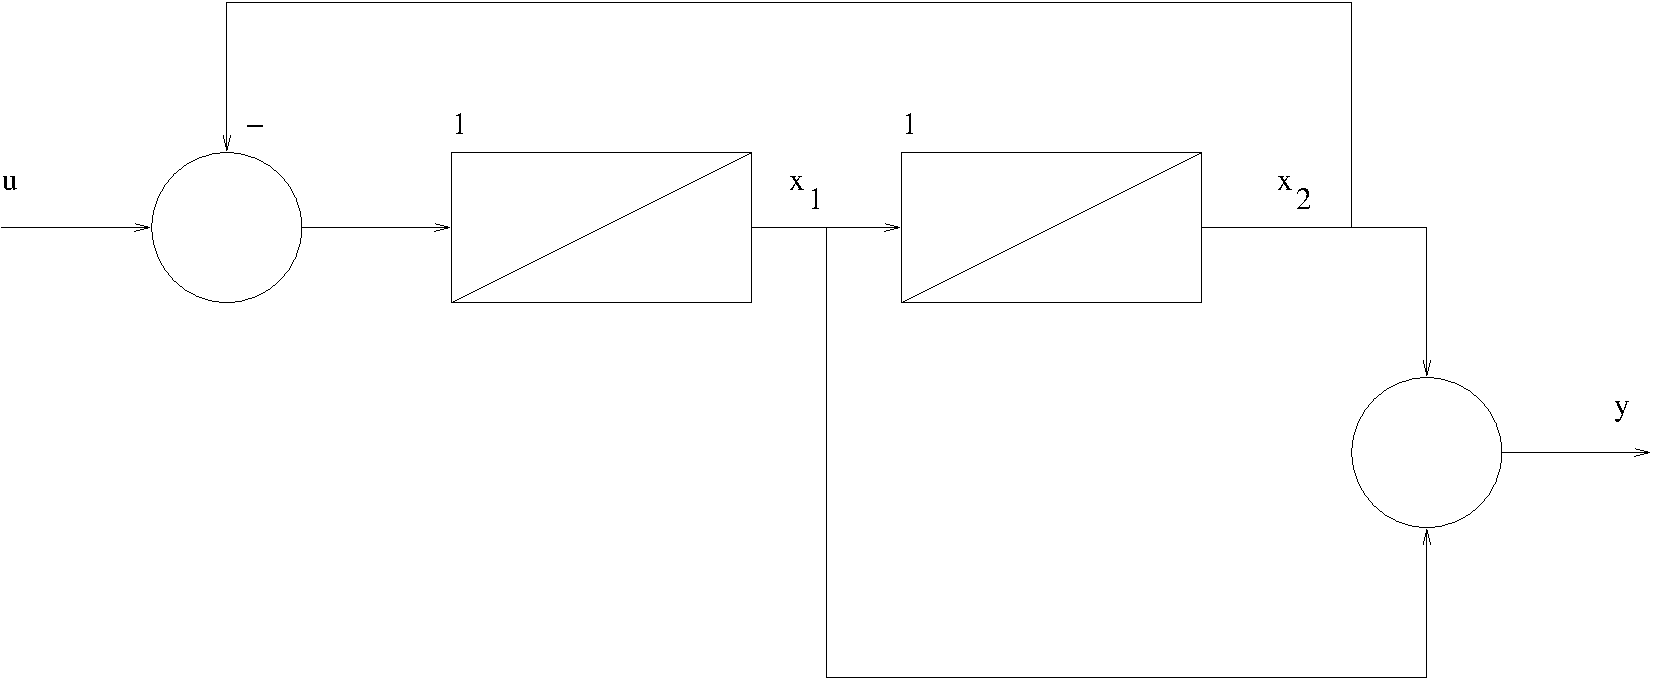
\includegraphics[height=5cm]{sysregel_bsp_2-3}
\end{figure}

\begin{align*}
  \begin{array}{llllllll}
    y(t)&=&x_1(t)+x_2(t)\\
    x_2(t)&=&\int{x_1(\tau)d\tau}&\Rightarrow&\dot{x_2}(t)&=&x_1(t)\\
    x_1(t)&=&\int{u(\tau)-x_2(\tau)d\tau}&\Rightarrow&\dot{x_1}(t)&=&&-x_2(t)+u(t)
  \end{array}
\end{align*}
\textbf{Vektoriell:}
\begin{align*}
  \begin{array}{lllll}
    \vec{\dot{x}}(t)&=&
    \begin{pmatrix}
      \dot{x_1}(t)\\
      \dot{x_2}(t)
    \end{pmatrix}
=
\begin{pmatrix}
  0&-1\\
  1&0
\end{pmatrix}
\cdot
\begin{pmatrix}
  x_1(t)\\
  x_2(t)
\end{pmatrix}
+
\begin{pmatrix}
  1\\0
\end{pmatrix}
u(t)\\[1cm]
\vec{\dot{x}}(t)&=&
\underbrace{
\begin{pmatrix}
  0&-1\\
  1&0
\end{pmatrix}}_{\mathbf{A}}
\vec{x}(t)+
\underbrace{
\begin{pmatrix}
1\\0  
\end{pmatrix}}_{\mathbf{B}}u(t)\\[1cm]
\vec{y}(t)&=& \underbrace{
  \begin{pmatrix}
    1&1
  \end{pmatrix}}_{\mathbf{C}}\vec{x}(t)\\
\mathbf{D}&=& \mathbf{0}
  \end{array}
\end{align*}

\paragraph{Aus der Differentialgleichung}
\begin{equation*}
y^{(n)}(t)+\dots+a_1\dot{y}(t)+a_0y(t)=b_0u(t)+b_1\dot{u}(t)+\dots+b_{n-1}u^{(n-1)}(t)  
\end{equation*}
(mit $a_n=1, b_n=0$, sonstige $a_i, b_j$ beliebig!)\\
Nach höchster Ableitung auflösen:
\begin{equation*}
  \Rightarrow y^{(n)}(t)=\underbrace{\underbrace{\underbrace{[b_0u(t)-a_0y(t)]}_{=\dot{x_1}(t)}+[b_1\dot{u}(t)-a_1\dot{y}(t)]}_{=\ddot{x_2}(t)}+\dots+[b_{n-1}u^{(n-1)}(t)-a_{n-1}y^{(n-1)}(t)]}_{=x_n^{(n)}(t)\Rightarrow y(t)=x_n(t)}
\end{equation*}
\begin{align*}
  \begin{array}{lllll}
    &y(t)&=&x_n(t)(**) \\
    \Rightarrow&\dot{x_1}(t)&=&-a_0x_n(t)+b_0u(t)\\
    &\dot{x_2}(t)&=&x_1-a_1x_n(t)+b_1u(t)\\
    &&\vdots\\
    &\dot{x_n}(t)&=&x_{n-1}-a_{n-1}x_n(t)+b_{n-1}u(t)
  \end{array}
\end{align*}
\textbf{Vektoriell:}
\begin{equation*}
  \vec{\dot{x}}(t)=
  \begin{pmatrix}
    0&0&\dots&0&-a_0\\
    1&0&\dots&0&-a_1\\
    0&1&\dots&0&-a_2\\
    \vdots&\vdots&\ddots&\vdots&\vdots\\
    0&0&\dots&1&-a_{n-1}
  \end{pmatrix}
\vec{x}(t)+
\begin{pmatrix}
  b_0\\
  b_1\\
  b_2\\
\vdots\\
  b_{n-1}
\end{pmatrix}
u(t)
\end{equation*}

Aus $(**)$ folgt damit durch Integrieren von $x_n(t)$
\begin{equation*}
  y(t)=
  \begin{pmatrix}
    0&0&\dots&0&1
  \end{pmatrix}
\vec{x}(t)
\end{equation*}

\section{Systembeschreibung im Bildbereich}

\subsection{Laplace-Transformation}

\subsubsection{Grundlagen}

\begin{description}
\item[Idee:] Die Lösung einer algebraischen Gleichung ist einfacher als Lösung einer DGL. Allerdings ist eine Transformation notwendig.
  \begin{align*}
    \begin{array}{lllll}
    Y(s)&=&\mathcal{L}\{y(t)\} &=& \int\limits_0^\infty{y(t)e^{-st}dt}\\
    y(s)&=&\mathcal{L}^{-1}\{Y(s)\} &=&\frac{1}{2\pi j} \int\limits_{c-j\infty}^{c+j\infty}{Y(s)e^{ts}ds}
    \end{array}
  \end{align*}
\end{description}
\begin{figure}[H]
  \centering
  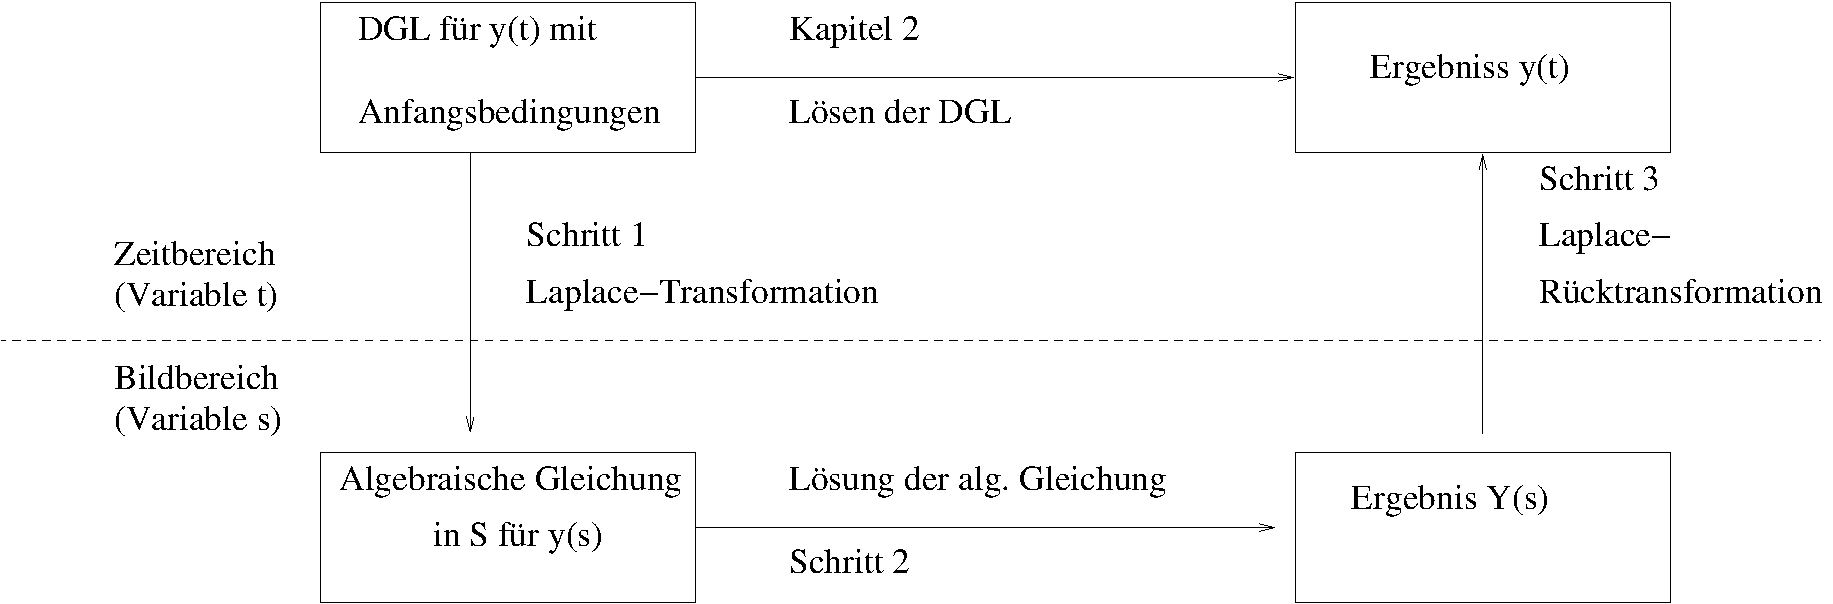
\includegraphics[width=\linewidth]{sysregel_laplace}
\end{figure}
\textbf{Vorraussetzung}
  \begin{enumerate}
  \item Es muss $y(t)=0$ für $t<0$ sein! Ansonsten stimmt das Modell nicht mit der Realität überein, das System würde antworten, \emph{bevor} ein Eingang angelegt ist. Schreibweise am besten: $y(t)\cdot \sigma (t)$\\
$y(t)$ kann Gewichtsfunktion eines Systems sein $\Rightarrow$ System ist kausal!

\item Das uneigentliche Integral muss konvergieren.
  \end{enumerate}
Der ``Umweg'' wird durch tabellierte Korrespondenzen attraktiv. Im Allgemeinen ist die Rücktransformation am aufwendigsten, da die Lösung aufgespalten und in Teilen transformiert werden muss.

\subsubsection{Lösung einer DGL}
\begin{bsp}[Sprungantwort eines $PT_1$-Gliedes]
\end{bsp}
\textbf{DGL:}
\begin{equation*}
  T\dot{y}(t)+y(t)=ku(t)
\end{equation*}
mit $y(0)=y_0$ und $u(t)=u_0\sigma (t)$
\begin{description}
\item[Schritt 1: ] Regel 1 und Regel 5
  \begin{equation*}
    T\cdot (sY(s)-y_0))+Y(s)=k\cdot U(s)
  \end{equation*}
$\Rightarrow$ Eingangssignal: Regel 1, Korr. 2

\begin{equation*}
U(s)=u_0 \cdot \frac{1}{s}
\end{equation*}

\item[Schritt 2:] Nach $Y(s)$ auflösen
  \begin{align*}
    \begin{array}{llllll}
      Y(s)(sT+1)&=&kU(s)+Ty_0\\
      Y(s)&=& \frac{T}{sT+1}y_0+\frac{k}{sT+1}u(s)\\
      \text{mit } U(s)&=&u_0\cdot \frac{1}{s}\\
      Y(s)&=&\underbrace{\frac{T}{sT+1}y_0}_{Y_1(s)}+\underbrace{\frac{k}{sT+1}\cdot \frac{u_0}{s}}_{Y_2(s)}
    \end{array}
  \end{align*}
\item[Schritt 3:] Rücktransformation
  \begin{equation*}
    Y_1(s)=\frac{1}{s+\frac{1}{T}}y_0 
  \end{equation*}
mit Korr. 6:
\begin{equation*}
  Y_1(t)=e^{-\frac{1}{T}t}\cdot y_0 \cdot \underbrace{\sigma (t)}_{=0 \text{ für }t<0} 
\end{equation*}
Partialbruchzerlegung für $Y_2(s)$:
\begin{equation*}
\frac{k u_0}{(sT+1)s}=\frac{A}{sT+1}+\frac{B}{s}
\end{equation*}
\begin{equation*}
  \Rightarrow k\cdot u_0=A\cdot s+B(sT+1)
\end{equation*}
\end{description}

\textbf{HIER FEHLT WAS!!!!}

\subsection{Übertragungsfunktion ÜF}

aus Bsp 3.1 :
\begin{equation*}
  Y(s)= \underbrace{\frac{T}{sT+1}y_0}_{\text{nur vom Anfangswert abh. Freie Bewegung}} + \underbrace{\frac{k}{sT+1}u(s)}_{\text{vom Eingang U(s) abh. Erzwungene Bew.}:=G(s)}
\end{equation*}
$G(s)$ heißt \emph{Übertragungsfunktion}. Sie beschreibt dsa System vollständig. Das Übertragungsverhalten bei verschwindendem Anfangswert, also $y(s)=G(s)\cdot u(s)$ entspricht $y(t)=g(t)*u(t)$ im Zeitbereich. Es gilt also $G(s)=\mathcal{L}\{g(t)\}$. (Regel 9)\\
Im Bildbereich können Systeme sehr einfach verknüpft werden, z.B. durch Serienschaltungen:
\begin{align*}
  \begin{array}{lllll}
    V(s)&=&G_1(s)\cdot U(s)\\
    Y(s)&=&G_2(s)\cdot V(s)&=&G_2(s)\cdot G_1(s)\cdot U(s)
  \end{array}
\end{align*}
\textbf{Beziehung zwischen DGL und ÜF}\\
z.B. Beispiel 3.1:
\begin{equation*}
  \underbrace{T}_{a_1}\cdot \dot{y}(t) +\underbrace{1}_{a_0}y(t)=\underbrace{k}_{b_0}\cdot U(t)
\end{equation*}
\begin{equation*}
  G(s)=\frac{\overbrace{k}^{b_0}}{\underbrace{T}_{a_1}s+\underbrace{1}_{a_0}}
\end{equation*}
\textbf{allgemein:} DGL der Form\\
\begin{equation*}
  a_ny^{(n)}+a_{n-1}y^{(n-1)}+\dots +a_1\dot{y}(t)+a_0=b(u(t))+b_1\dot{u}(t)+\dots +b_mu^{(n)}(t)
\end{equation*}
$\Rightarrow$ Rationale ÜF (Regel 5 mit verschwindendem Anfangswert)
\begin{equation*}
  G(s)=\frac{Y(t)}{U(s)}= \frac{b_0+b_1\cdot s + b_ms}{\underbrace{a_0+a_1\cdot s +a_ns^n}_{\text{Nullstellen des Nenners }:=\text{ Pole der ÜF}}}
\end{equation*}
\begin{itemize}
\item Falls $n<m$: ``Reales'' System
\item Falls $n<m$: differenzierendes Verhalten
\item falls $a_0=a_1=\dots=a_\rho =0$: $s^\rho$ kann im Nenner ausgeklammert werden $\Rightarrow$ $\rho$-fach integrierend. 
\end{itemize}
\paragraph{praktische Betrachtung}
\begin{bsp}Harmonische Anregung eines Federschwingers
\end{bsp}
\subparagraph{Messungen}
\begin{figure}[H]
  \centering
  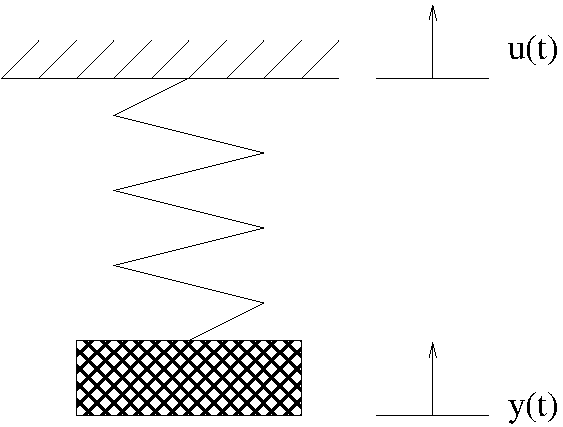
\includegraphics[width=0.4\linewidth]{sysregel_bsp_3-4}
\end{figure}
\begin{align*}
  \begin{array}{|l|c|l|l|l|l|l|l|l|l|}
    \hline
    \omega               &0,2 &0,4 &0,6 &0,8&1,0&1,2&1,4&2,0&10    \\
    T=\frac{2\pi}{\omega}&31,4&15,7&10,5&7,9&6,3&5,2&4,5&3,1&0,62  \\
    \hline
    A(\omega)            &1,04&1,16&1,45&2,1&2,5&1,5&0,9&0,3&0,01  \\
    \Phi(\omega)         &-\frac{0,4}{31,4}\cdot 360\degree =-4,5\degree&-9\degree&-17\degree&-45\degree&-90\degree&-139\degree&-160&-174&-180\\
\hline
  \end{array}
\end{align*}
\begin{itemize}
\item Der Frequenzgang $G(j\omega)=A(\omega)\cdot e^{j\Phi(\omega}$ wird in Stützstellen $\omega$ definiert
\item Damit ist auch die ÜF $G(s)$ definiert!
\item Graphische Darstellung? Die sog. \emph{Ortskurve} wird in Kap. 3.5 beschriegen, das sog. \emph{Bode-Diagramm} in Kap. 3.6
\end{itemize}

\subsection{Ortskurve}

Die Ortskurve ist ein Kurvenzug, der von $G(j\omega)$ in der komplexen Ebene beschrieben wird, wenn die Anregungsfrequenz $\omega$ im Intervall $(0\leq \omega \leq \infty)$ variiert wird.
Auftragen von $A(j\omega)$ in einem Zeigerdiagramm (Imaginärteil über Realteil). Durch anschließendes Verbinden der Punkte erhält man die sog. \emph{Ortskurve}.\\
Die Ortskurve kann auch aus $G(s)$ berechnet werden:
\begin{itemize}
\item I-Glied: $G(s)=k\cdot \frac{1}{s} \underbrace{\Rightarrow}_{s=j\omega}G(j\omega)=k\cdot \frac{1}{j\omega}=\underbrace{k\cdot \frac{1}{\omega}}_{A(\omega)=const.}\cdot \underbrace{e^{-j\frac{\pi}{2}}}_{\Phi(\omega)}$
\item $T_t$-Glied: $G(s)=k\cdot e^{-sT_t}; G(j\omega)=\underbrace{k}_{A(\omega)=const.}\cdot \underbrace{e^{-j\omega T_t}}_{\Phi(\omega)}$
\end{itemize}
Für eine Übersicht genügt die Betrachtung der Asymptoten der Ortskurve:
\[
G(j\omega)=\frac{b_0+b_1(j\omega)+\dots+b_m(j\omega)^m}{a_0+a_1(j\omega)+\dots+a_n(j\omega)^n}\cdot e^{-(j\omega)T_t}
\]

\paragraph{Anfang der Ortskurve:}

\begin{itemize}
\item falls $a_0 \neq 0, b_0 \neq 0$\\
  $\lim\limits_{w\mapsto 0}{G(j\omega)=\frac{t_0}{a_0}=k}$ Start der OK auf der Re-Achse
\item falls $a_0=a_1=\dots=a_{\rho -1}=0$ $\rho$-fach Integrierend\\
$\lim\limits_{\omega \mapsto 0}{G(j\omega)}= \lim\limits_{\omega \mapsto 0}{\frac{b_0+\dots+b^m}{a_\rho(j\omega)^\rho+\dots+a_n(j\omega)^n}}=\lim\limits_{\omega \mapsto 0} {\frac{1}{(j\omega)^\rho} \cdot \frac{b_0+\dots}{a_\rho+\dots}}=\lim\limits_{\omega \mapsto 0}{\frac{1}{\omega^\rho}\cdot \frac{b_0}{a_\rho}\cdot e^{-j\rho\frac{\pi}{2}}} \Rightarrow$ OK kommt aus dem Unendlichen mit Phasenwinkel $-\rho \frac{\pi}{2}$
\end{itemize}

\paragraph{Ende der Ortskurve:}

Das Ende der Ortskurve lässt sich analog zum Anfang über $\lim\limits_{\omega \mapsto \infty}{G(j\omega}$. Vgl. auch Skript S. 33
\begin{bsp}
\end{bsp}
$G_1(s)=\frac{s+2}{(s+1)^4}$ \\
mit $\omega =1;n=4;\rho=0;T_t=0$\\
$G_2(s)=\frac{1}{s+s^2}\cdot e^{-2s}$\\
mit $m=0;n=2;\rho=1;T_t=2$

\textbf{HIER FEHLEN BILDER UND EINE TABELLE}
\subsection{Bode-Diagramm}

\subsubsection{Definition}

Das Bode-Diagramm ist die getrennte graphische Darstellung des \emph{Amplitudenverlaufs $A(\omega)$} und des \emph{Phasenverlaufs $\Phi(\omega)$} über der Frequenz $\omega$. In der Regel werden die Größen logaritmisch aufgetragen.\\
Die Amplitude wird auch logaritmisch in Dezibel (dB) dargestellt:
\[
A(\omega)_{dB}=20 log_{10}A(\omega)
\]

\subsubsection{Bode-Diagramme häufig verwendeter Übertragungsglieder}

\paragraph{P-Glied}

\[
G(j\omega)=k\\
A(\omega)_{dB}=20\cdot \log{K}\\
\Phi(\omega)=0\degree
\]

\paragraph{I-Glied}

\[
G(j\omega)=\frac{k}{j\omega}=\frac{k}{\omega}\cdot e^{-j\frac{\pi}{2}}\\
\Rightarrow A(\omega)_{dB}=20\cdot \log{\frac{k}{\omega}}=-20 \log{\frac{\omega}{k}}\\
\Phi(\omega)=-90\degree=-\frac{\pi}{2}
\]
Nulldurchgang von A für $\frac{\omega}{k}=1$, also $\omega =k$\\
Amplitudenverlauf sinkt um 20 dB, wenn sich $\omega$  verzehnfacht.

\paragraph{$T_t$-Glied}

\[
G(j\omega)=k\cdot e^{-j\omega T_t} \text{ mit }k=1\\
\Rightarrow A(\omega)_{dB}=0\\
\Phi(\omega)=-\omega T_t
\]
Phasenverlauf sinkt linear mit der Frequenz $\omega$. Durch die logarithmische $\omega$-Achse wird der Phasenverlauf gestaucht. $\rightarrow$ Kurve aus den Stützstellen konstruieren! \\
$\Phi(\omega)$ ist normalerweise in Grad:
\[
\Phi(\omega)=-\omega T_t\cdot \frac{180\degree}{\pi}
\]
Es gilt $\omega = \omega_0 =\frac{1}{T_t}$
\[
\Phi(\omega_0)=-1\cdot \frac{180\degree}{\pi}=-57,3\degree
\]

\paragraph{$pT_1$-Glied}

\[
G(j\omega)=\frac{k}{1+j\omega T}\\
\text{mit } k=1 \text{ und } \omega_0=\frac{1}{T}\\
G(j\omega)=\frac{1}{1+j\frac{\omega}{\omega_0}}\\
A(\omega)=|G(j\omega)|=\frac{1}{\sqrt{1+(\frac{\omega}{\omega_0})^2}}
\]
$\omega_0$:Eckfrequenz
\begin{itemize}
\item für $\omega << \omega_0$: $A(\omega)\approx 1 =0dB$
\item für $\omega=\omega_0$: $A(\omega)=\frac{1}{\sqrt{2}}= -3dB$
\item für $\omega >>\omega_0$: $A(\omega)\approx \frac{\omega_0}{\omega}$\\
  $\Rightarrow A(\omega)_{dB}=20\log{\frac{\omega_0}{\omega}}=-20\log{\frac{\omega}{\omega_0}}$
\[
G(j\omega)\underbrace{=}_{\text{konj. kompl. erweitern}} \frac{1-j\frac{\omega}{\omega_0}}{1+(\frac{\omega}{\omega_0})^2}\\
\Rightarrow \Phi(\omega)=\arctan{\frac{Im(G(j\omega))}{Re(G(j\omega))}}\\
 =\arctan{\frac{-\frac{\omega}{\omega_0}}{1}}=-\arctan{\frac{\omega}{\omega_0}}
\]
\end{itemize}
\textbf{HIER FEHLT WAS!!!}

\paragraph{$pT_2$-Glied}

$\rightarrow$ Blatt 1-10
\begin{bsp}
\end{bsp}
Parameter aus dem Bode-Diagramm ablesen:$\omega_0 \approx 1 \rightarrow T=\frac{1}{\omega}=1$
\textbf{Auch hier fehlt was}
\subsubsection{Rechenregeln}

\paragraph{Serienschaltung}

\textbf{Hier fehlt dsa bild}
\[
G(j\omega)=G_1(j\omega)\cdot G_2(j\omega)\cdot \dots \cdot G_n(j\omega)
\]
mit $G_i = A_i(\omega)e^{j\Phi_i(\omega)}$\\
\[
G(j\omega)=\underbrace{A_1(\omega)\cdot A-2(\omega)\cdot \dots \cdot A_n(\omega)}_{A(\omega)}\cdot e^{j\underbrace{(\Phi_1(\omega)+\Phi_2(\omega)+\dots + \Phi_n(\omega))}_{\Phi(\omega)}}
\]
\begin{bsp}
\end{bsp}

\paragraph{P-Glied}
\[
G(j\omega)=\frac{10\cdot(1+2j\omega)}{(1+10j\omega)(1+0.2j\omega)}=\frac{10\cdot (1+j\frac{\omega}{0.5})}{(1+j\frac{\omega}{0.1})(1+j\frac{\omega}{5})}
\]
\textbf{Logaritmische Plots fehlen}

\section{Analyse von Systemeigenschaften}

\subsection{Stabilität}

\subsubsection{Definitionen und Bedingungen}

\begin{bsp}
Pendel
\end{bsp}
\begin{figure}[H]
  \centering
  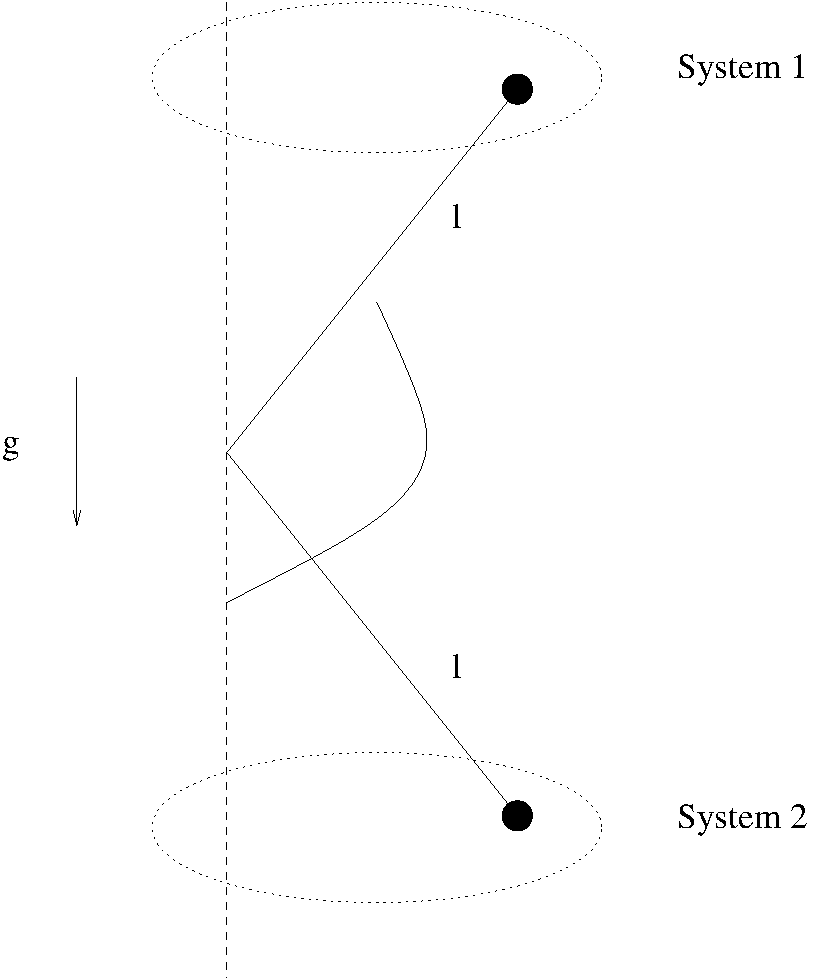
\includegraphics[width=0.4\linewidth]{sysregel_bsp_4_1}
\end{figure}
\textbf{Linearisierung oben und unten, mitte DGL}
Gesucht ist der Zeitverlauf der Systeme bei beliebigen Anfangsbedingungen.

\begin{description}
\item[System 1]
\[\ddot{\phi}+d\dot{\phi}-\frac{g}{l}\phi=0\]
Homogene Lösung:
\[
s^2+ds-\frac{g}{l}=0
\]
$\Rightarrow s_{1,2}=-\frac{d}{s}\pm \sqrt{(\frac{d}{2})^2+\frac{g}{l}}$\\
$\Rightarrow s_{1,2}$ sind reel, z.B. $s_1 < 0, s_2 >0$\\
Ansatz: $\phi(t)=C_1e^{s_1t}+C_2e^{s_2t}$. Ein Anteil geht also gegen 0, der andere gegen $\infty$. Man nennt solche Systeme \emph{instabil}.
\item[System 2] 
Analog oben. Die lösungen sind komplex oder reel, und größer $\frac{d}{2}$. Beim Ansatz gehen nun beide Anteile gegen 0. Man nennt solche Systeme \emph{stabil}.
\item[System 3] $d=0 \rightarrow $ Keine Dämpfung. Homogene Lösung:
\[
s^2+\frac{g}{l}=0
\] 
$S_{1,2}=\pm \sqrt{-\frac{g}{l}}=\pm j\sqrt{\frac{g}{l}}$\\
Ansatz: $\phi(t)=C_1\cos{\sqrt{\frac{g}{l}}t}+C_2\sin{\sqrt{\frac{g}{l}}t}$\\
Betragsmäßig gesehen sind die Anteile stets größer oder gleich der jeweiligen Konstante. Das System strebt also gegen keinen Endwert, bleibt aber beschränkt. Man nennt solche Systeme \emph{grenzstabil}.\\
Die Stabilität wird als eine \emph{Systemeigenschaft} definiert, die nicht von der Art der Anregung abhängt. 

\end{description}
\begin{itemize}
\item Das System ist durch die Gewichtsfunktion $g(t)$ gegeben.\\
 Die Anfangsanregung für $t>0, u(t)=0$ ist gegeben durch:
\[u(t)=C\cdot \delta (t) \]
\[
\Rightarrow y(t)=g(t)*u(t)=\int\limits_0^t{g(\tau)u(t-\tau)d\tau}= C\cdot \int\limits_0^t{g(\tau)\delta(t-\tau)}=C\cdot g(t)
\]
Die Stabilitätsdefinition für y(t) ist auch auf g(t) anwendbar, z.B. falls $g(t)\mapsto o$ für $t\mapsto \infty \Rightarrow$ stabil
\item Das System ist durch die ÜF G(s) gegeben:\\

Man bestimmt die Polstellen der ÜF. Das System heißt
\begin{itemize}
\item instabil, sobald für einen Pol gilt $Re(s_i)>0$
\item stabil, sobald alle Pole $s_i$nur Realteil haben $Re(s_i)<0$
\item grenzstabilm sobald für einen Pol $S_i$ gilt $Re(S_i)=0$
\item Einen Sonderfall bildet ein mehrfacher Pol mir $Re(S_i)=0$. z.B. $s_1=s_2=0$:
$G(s)=\frac{1}{s^2}$, $g(t)=t\cdot \sigma(t)$.\\
$\lim\limits_{t\mapsto \infty}{g(t)=\infty} \Rightarrow$ instabil! 
\end{itemize}
\item Das System ist im  Zustandsraum gegeben:
\[
\dot{y}(t)=\mathbf{A}\vec{x}(t)
\]
mit $\vec{u}(t)=0$ und $\vec{x}(0)=\vec{x_0}$ beliebig.
\begin{itemize}
\item Ein Sonderfall existiert, wenn der Zustandsvektor ein Skalar ist:
\[
\dot{x}(t)=ax(t)\Rightarrow \dot{x}(t)-ax(t)=0
\]
Hier lautet die homogene Lösung
\[
s-a=0 \Rightarrow s_1=a
\]
\[
x(t)=Ce^{at}
\]
$\Rightarrow$ stabil für $Re(a)<0$
\item Verallgemeinerung (ohne Beweis!)\\
Das dynamische System 
\[
\vec{\dot{x}}(t)=\mathbf{A}\vec{x}(t)+\mathbf{B}\vec{u}(t)
\] 
ist stabil, wenn für sämtliche Eigenwerte $S_i$ $i=1\dots n)$ der Systemmatrix$\mathbf{A}$ gilt: $Re(s_i)<0$
\end{itemize}
\end{itemize}

\subsubsection{Hurwitz-Kriterium}

\[
G(s)=\frac{Z(s)}{a_0+a_1s+\dots+a_ns^2}=\frac{Z(s)}{(s-s_1)(s-s_2)\dots (s-s_n)}
\]
Die $s_i$ bestimmen die Stabilität. Gesucht ist ein einfaches Stabilitätskriterium, welches die zum Teil aufwändige Faktorzerlegung (s.o.) nicht erfordert.
\begin{enumerate}
\item Notwendige Bedingung:\\
$(s-s_1)(s-s_2)\dots (s-s_n)=0$.\\
Es gibt davon $Z_q$ konjugiert komplexe Wurzelpaare:\\
$s_{2k-1,2k}=\sigma_{2k}\pm j\omega_{2k}$ mit $k=1\dots q$.\\
Für asymptotische Stabilität muss gelten. \\
$\sigma_k<0$ bzw. $\sigma_k=-|\sigma_k|$ für $k=1,\dots, n$. \\
Nach einsetzen und ausmultiplizieren ergeben sich nur positive koeffizienten vor $s_i$. Dies ist die notwendige Bedingung für stabilität!
\item Hinreichende Bedingung (am Beispiel n=4):
\[
a_0+a_1s+a_2s^2+a_3s^3=0
\]
Die Stabilitätsgrenze ist die imaginäre Achse. Es wird also $s=j\omega$ eingesetzt:
\[
a_0+a_1j\omega+a_2(j\omega)^2+a_3(j\omega)^3=0
\]


\begin{itemize}
\item Re: $a_0-a_2\omega^2=0\Rightarrow \omega^2=\frac{a_0}{a_2}$
\item Im: $a_1\omega -a_3\omega^3=0\Rightarrow a_1-a_3\omega^2=0\Rightarrow a_1-a_3\frac{a_0}{a_2}=0$\\
$a_2\neq0 \Rightarrow a_1a_2-a_3a_0=0$ 
\end{itemize}
Auf welcher Seite der Grenze ist dsa System stabil?\\
Das System ist stabil, falls \[a_1a_2-a_3a_0>0\]
Die allgemeine Form findet sich im Skript auf Blatt 4-2 und 4-3
\end{enumerate}
\begin{bsp}
\end{bsp}
\[
G(s)=\frac{1}{s^3+2s^2+8s+1+h}
\]
Für welche k ist dsa System stabil?\\
\begin{enumerate}
\item Alle $a_i$ müssen größer 0 sein. $1+k>0 \Rightarrow k>-1$
\item $a_1a_2-a_3a_0>0$:\\
$\Rightarrow 2\cdot 8-1(1+k)=15-k>0$\\
$k<15 \Rightarrow$ stabil für $-1<k<15$
\end{enumerate}

\subsubsection{Nyquist-Kriterium}

\begin{itemize}
\item speziell für rückgekoppelte Systeme
\item anders als Hurwitz-Kriterium ist es auch für Systeme mit Totzeit geeignet.
\end{itemize}

\begin{figure}[H]
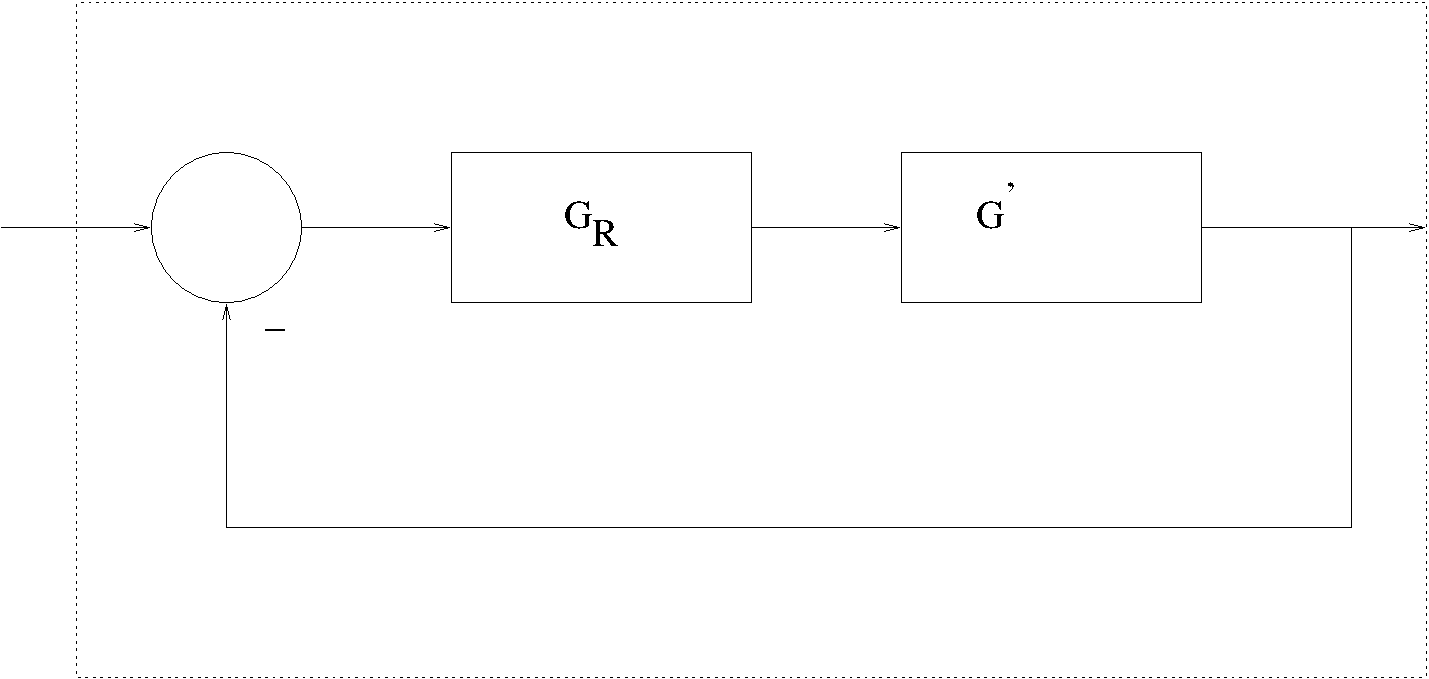
\includegraphics[width=0.7\linewidth]{sysregel_nyquist}
\end{figure}
Kriterium für einfache Fälle:\\
Der \emph{geschlossene} Kreis ist stabil, falls die Ortskurve des \emph{offenen} Kreises den kritischen Punkt $-1$ links liegen lässt. $\rightarrow$ Blatt 4-4

\begin{bsp}
\end{bsp}
\[
G_0(s)=\frac{k}{(1+s)^3}
\]
wird rückgekoppelt. Für welche K ist das System stabil?
\begin{figure}[H]
  \centering
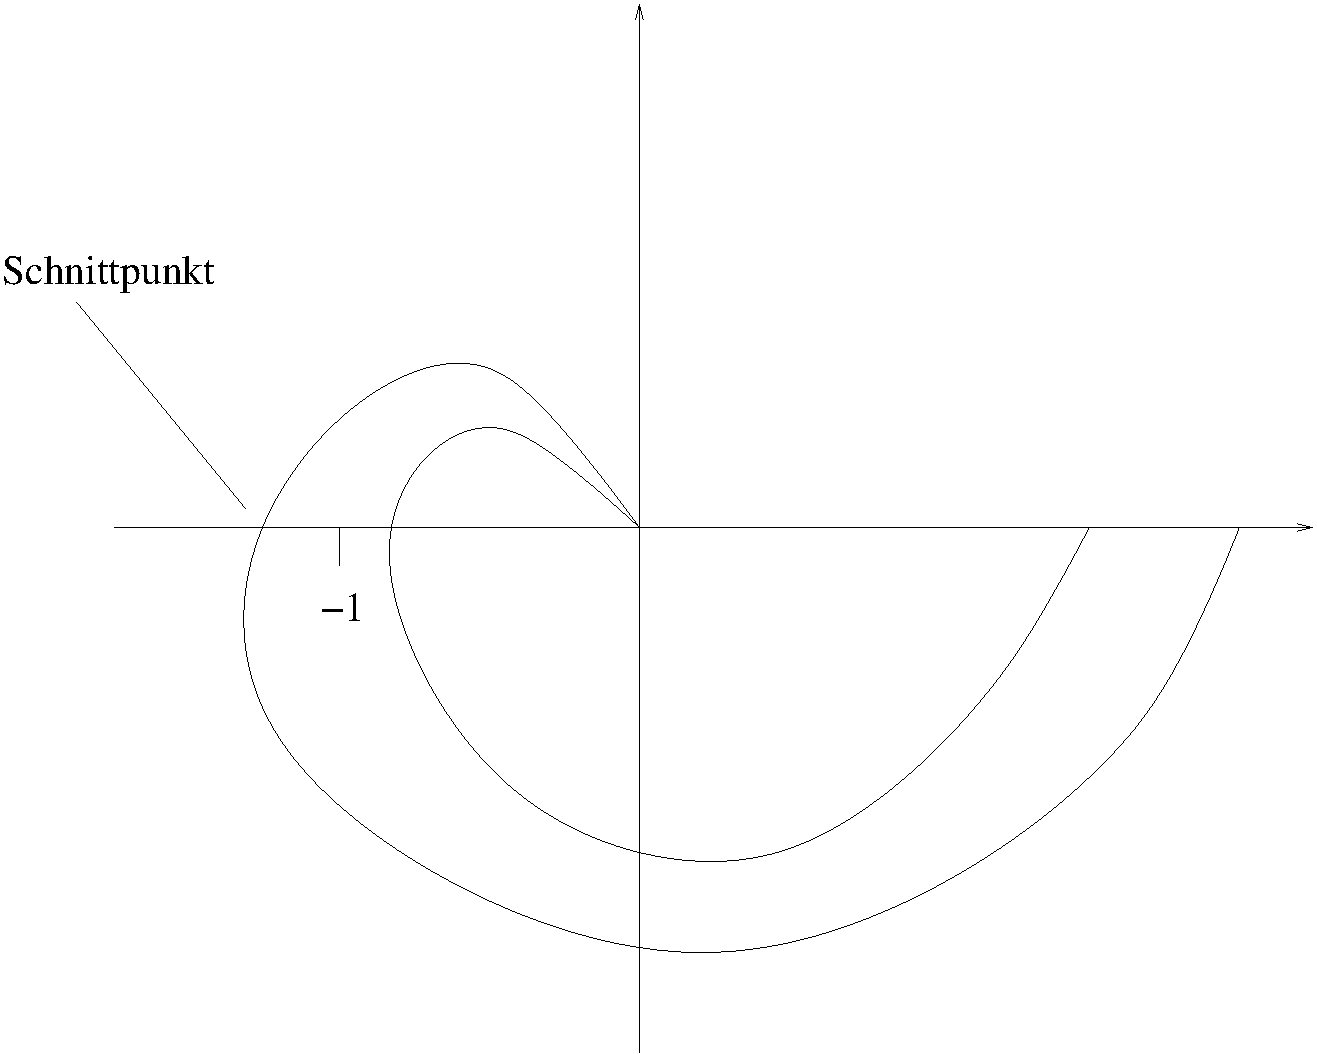
\includegraphics[width=.5\linewidth]{sysregel_bsp_4_3}  

\end{figure}
\begin{itemize}
\item Berechnung des Schnittpunktes

$G_0(j\omega)$ ist reel, wenn der Nenner reell ist:
\[
(1+j\omega)^3=1+3j\omega-3\omega^2-j\omega^3
\]
Für dem Imaginärteil muss also gelten: $3\omega-\omega^3=0$. Da $\omega$ zusätzlich immer größer als 0 ist, gilt: $3-\omega^2=0 \rightarrow \omega_0^2=3$
\item $w_0$ in die Übertragungsfunktion einsetzen, mit der Stabilitätsbedingung $G<-1$
\[
G_0(j\omega_0)=\frac{k}{1-3\cdot 3}>-1 \Rightarrow k<8
\] 
Das Nyquist-Kriterium kann analog im Bodediagramm angewandt werden:\\
$\Rightarrow$ bei $\Phi(\omega)=-180\degree$ muss gelten $A(\omega)<0dB$
\end{itemize}

\subsection{Steuerbarkeit}

Im folgenden Kapitel 5 sollen dynalische Systeme durch einen Regler dynamisch korrigiert werden, indem sie über ihre Eingänge geeignet angesteuert werden.\\
Unter welchen Vorraussetzungen gelingt das?
\begin{itemize}
\item Die Eingänge $u(t)$ müssen auf alle Systemteile wirken können.
\item Ein System heißt dann \emph{steuerbar}. (vgl Blatt 4-6)
\end{itemize}

\paragraph{BSP:}

\begin{figure}[H]
  \centering
  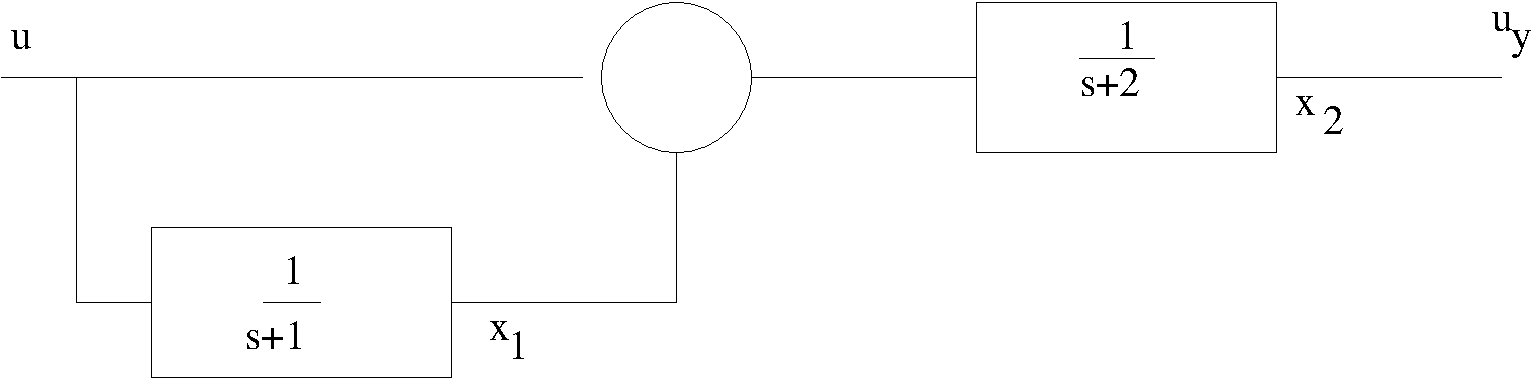
\includegraphics[width=.7\linewidth]{sysregel_bsp_kap4}
\end{figure}
Ist dieses System steuerbar?
\[
x_1(s)=\frac{1}{(s+1)}\cdot u(s);x_2(s)=\frac{1}{s+2}\cdot (U(s)+x_1(s))
\]
\[
sx_1(s)=-x_1(s)+u(s);sx_2(s)=x_1(s)-2x_2(s)+u(s)
\]
\[
\dot{x_1}(t)=-x_1(t)+u(t);\dot{x_2}(t)=x_1(t)-2x_2(t)+u(t)
\]
\[
\begin{pmatrix}
\dot{x_1}\\
\dot{x_2}
\end{pmatrix}
=
\underbrace{\begin{pmatrix}
 -1&0\\
 1&-2 
\end{pmatrix}}_{\mathbf{A}}
\cdot
\begin{pmatrix}
  x_1(t)\\
  x_2(t)
\end{pmatrix}
+
\underbrace{\begin{pmatrix}
  1\\
1
\end{pmatrix}}_{\mathbf{B}}
\cdot u(t)
\]

Steuerbarkeitsmatrix:
\[
Q_s=
\begin{pmatrix}
  \mathbf{B},\mathbf{A}\mathbf{B}
\end{pmatrix}
=
\begin{pmatrix}
  1&-1\\
1&-1
\end{pmatrix}
\]
Berechnung des Ranges der Matrix:
\[
rang(Q_s)=1 \neq u=2\Rightarrow \text{ \emph{Nicht} steuerbar}
\]
\begin{description}
\item[Erklärung] $G(s)=\frac{s+2}{s+1}\cdot\frac{1}{s+2}=\frac{1}{s+1}\rightarrow $ Ordnung=1\\
$\Rightarrow$ Das System besitzt keine zwei Freiheitsgrade!
\end{description}

\subsection{Beobachtbarkeit}

Um ein System beherrschen zu können, müssen alle inneren Zustände auf die Ausgangsgröße $y(t)$ wirken. Ein solches System heißt \emph{Beobachtbar} (vgl. Blatt 4-2)
\begin{figure}[H]
\begin{bsp}
\end{bsp}
\centering
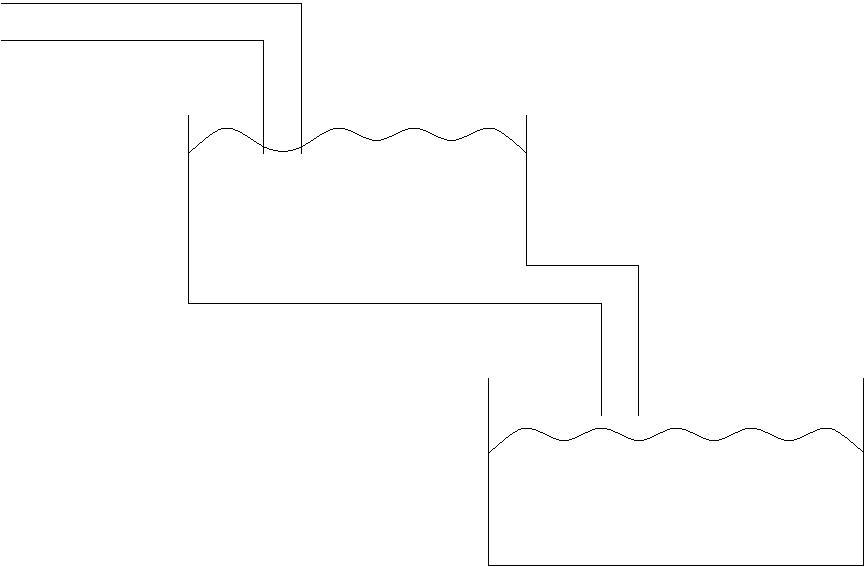
\includegraphics[width=.4\linewidth]{sysregel_bsp_4_2}
\end{figure}
Bilanzen:
\[
\dot{h_1}(t)=-kh_1(t)+q(t)
\]
\[
\dot{h_2}(t)=kh_1(t)-kh_2(t)
\]
o.B.d.A. sei k=1
\[
\Rightarrow
\begin{pmatrix}
  \dot{h_1}(t)\\
\dot{h_2}(t)
\end{pmatrix}
=
\begin{pmatrix}
  -1&0\\
1&-1
\end{pmatrix}
\cdot
\begin{pmatrix}
  h_1(t)\\
h_2(t)
\end{pmatrix}
+
\begin{pmatrix}
  1\\0
\end{pmatrix}
\cdot q(t)
\]

Sollte der Füllstandssensor sinnvollerweise am Behälter 1 oder am Behälter 2 installiert werden?\\
Behälter 1:
\[
Q_B=
\begin{pmatrix}
  \mathbf{C}\\
\mathbf{CA}
\end{pmatrix}
=
\begin{pmatrix}
  1&0\\
-1&0
\end{pmatrix}
\]
Behälter 2 analog:
\[
Q_B=
\begin{pmatrix}
  0&1\\
1&-1
\end{pmatrix}
\]
Der Rang der Matrix von Behälter 1 ist 1, das System ist also nicht beobachtbar. Der Rang von Behälter 2 ist 2 und damit gleich u, somit ist dsa System beobachtbar. Man sollte den Sensor also an Behälter 2 anbringen.


\section{Reglerentwurf}

\begin{description}
\item[Idee] Aus dem Sollwert und der fortlaufenden Beobachtung des dynamischen Systems (``Strecke'') wird eine geeignete Änderung des Systems (``Stellgröße'') bestimmt, die dazu führt, das der Ausgangswert des Systems (``Regelgröße'') dem Sollwert folgt. Dies geschiet auch bei Störeinwirkung.
\end{description}

\subsection{Reglerentwurf im Bildbereich}
\begin{figure}[H]
  \centering
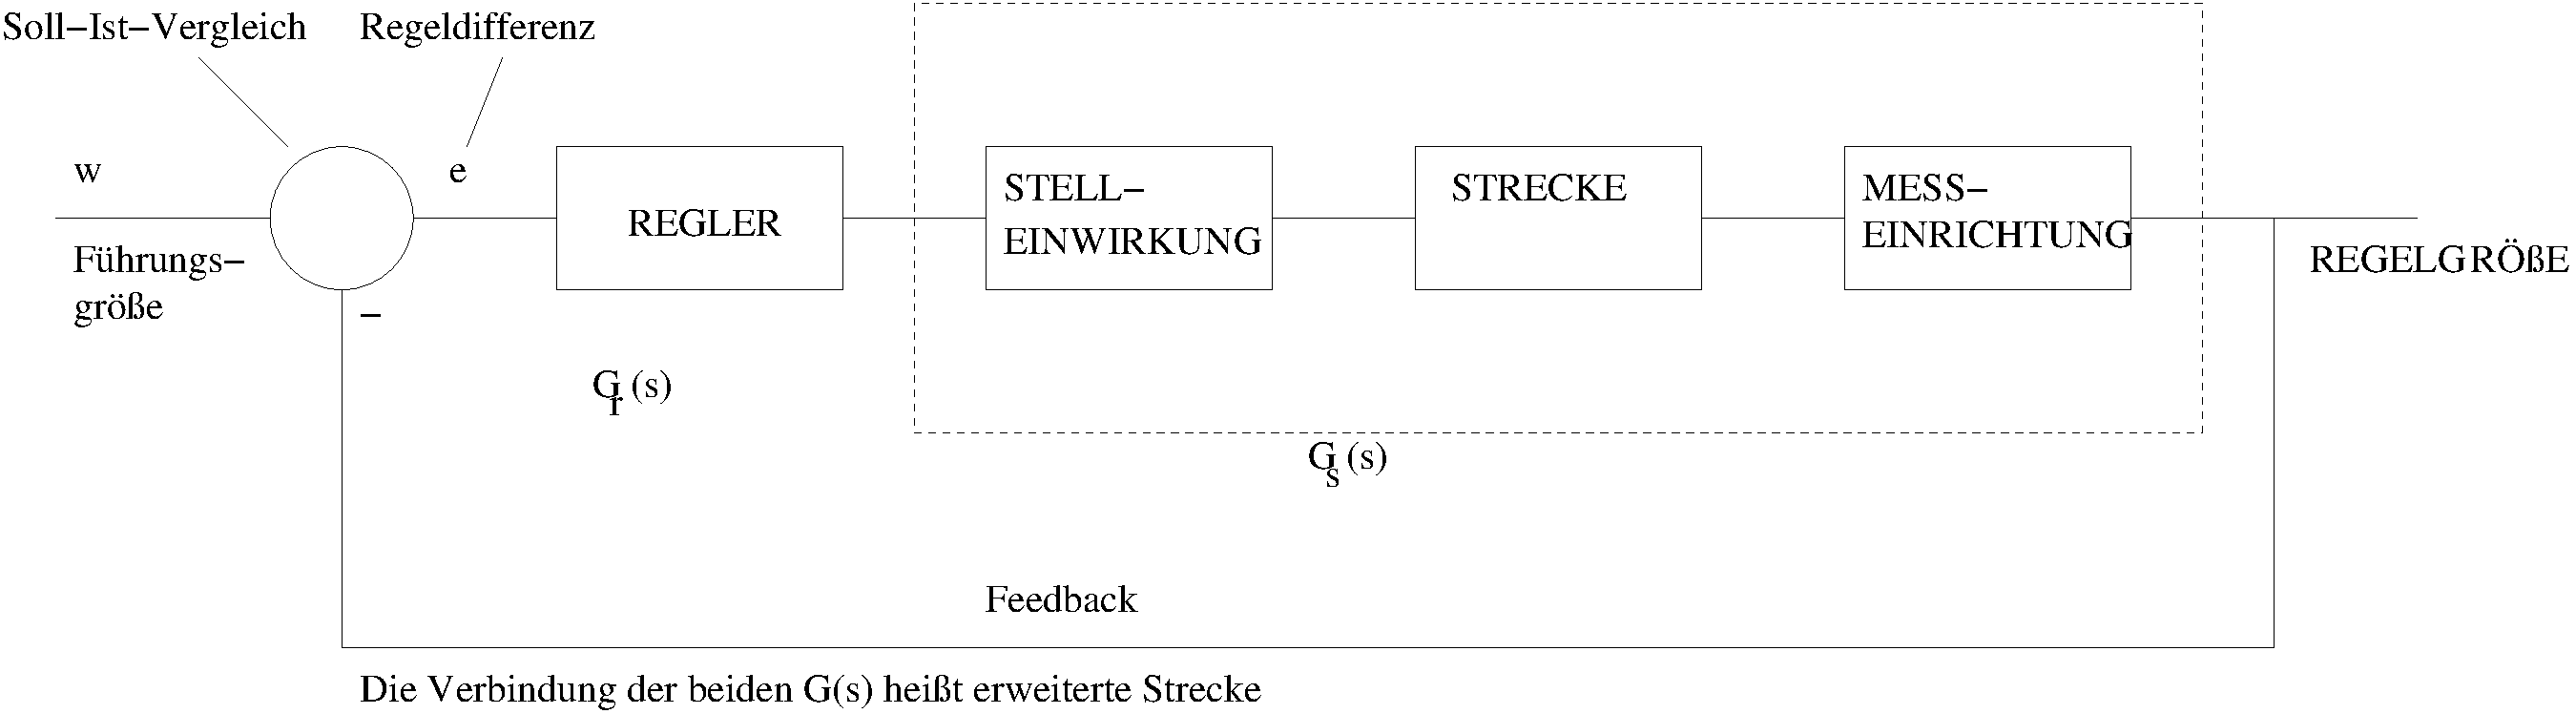
\includegraphics[width=\linewidth]{sysregel_regler}  

\end{figure}

Beispiele für Regler sind z.B. in einem Spülkasten  oder in einer Wohnraumheitzung zu finden.
\begin{table}[H]
  \centering
  \begin{tabular}{|l||l|l|l|l|l|l|}
\hline    
 System&Führungsgr.&Regler&Stelleinricht.&Strecke&Messeinricht.&Regelgr.\\
\hline
\hline
Spülkasten&Sollhöhe&Ventil&--------------&Spülkasten&Schwimmer&Füllhöhe\\
\hline
Heizung&Handrad&Ventil&Heizkörper&Wohnraum&Thermometer&Raumtemp.\\
\hline
  \end{tabular}
\end{table}
\begin{description}
\item[Führungsverhalten] Die Regelgröße y(t) soll der Führungsgröße w(t) möglichst gut folgen. \\
Führungs-Übertragungsfunktion:
\[
\frac{Y(s)}{w(s)}=G_w(s)
\]
\begin{align*}
  \begin{array}{lll}
    Y(s)&=&w(s)\cdot G_R(s)\cdot G_s(s)-Y(s)\cdot G_R(s)\cdot G_S(s)\\
    Y(s)\cdot [1+G_R(s)\cdot G_S(s)&=&G_S(s)\cdot G_R(s)\cdot w(s)\\
  \end{array}
\end{align*}

\[G_w(s)=\frac{Y(s)}{w(s)}=\frac{G_s(s)\cdot G_R(s)}{1+G_S(s)\cdot G_R(s)}=\frac{G_0(s)}{1+G_0(s)}\stackrel{!}{=}1 \text{ (ideales Führungsverhalten)}
\]
mit $G_0(s)$: erweiterte Strecke.\\
$\lim\limits_{t\mapsto \infty}{y(t)}=w=const. \rightarrow $ Regelkreis stationär genau

\item[Störverhalten] Die meist unbestimmte Störung z(t) soll möglichst keine Wirkung auf das System haben. Analog zum Führungsverhalten mit $z_1$: Additive Störung\\
Störungs-Übertragungsfunktion:

\[
G_{z_1}(s)=\frac{Y(s)}{Z_1(s)}=\frac{G_s(s)}{1+G_s(s)\cdot G_R(s)}\stackrel{!}{=}0 \text{ (ideales Störverhalten)}
\]
Im Allgemeinen kann eine Störung am Ende des Regelkreises schlechter ausgeglichen werden als eine Störung am Anfang des Regelkreises.
\end{description}

\textbf{HIER FEHLT NOCH 5.1.1}

\subsubsection{Fehlt noch}
\subsubsection{Forderungen für die Reglersynthese}
\begin{itemize}
\item[\RM{1}] \underline{Der Regelkreis soll stabil sein!}\\
Überprüfung durch
\begin{itemize}
\item Hurwitz-Kriterium (geschlossener Kreis $G_w(s)$!)
\item Nyquist-Kriterium (offener Kreis $G_0(s)-G_R(s)G_s(s)$ (Auch für Systeme mit Totzeit)
\end{itemize}
\item[\RM{2}] \underline{Der Regelkreis muss genügend stationäre Genauigkeit besitzen!}\\
\textbf{Beispiel:} Die Strecke
\[
G_s(s)=\frac{0.1}{(1+10s)(1+5s)(1+2s)}
\]
soll durch ein P-Glied mit $G_R(s)=K_R$ geregelt werden.
\begin{figure}[H]
  \centering
  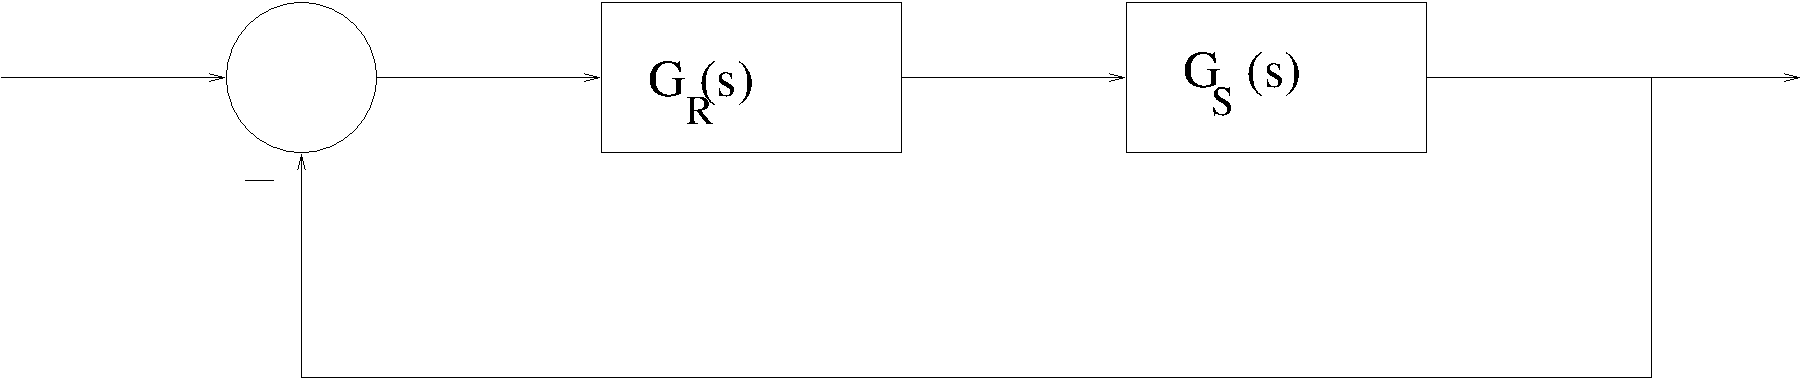
\includegraphics[width=.7\linewidth]{sysregel_No_1}
\end{figure}

Nach (\RM{1}): geschlossener Kreis
\begin{align*}
  \begin{array}{llllll}
    G_w(s)&=&\frac{G_0(s)}{1+G_0(s)}&=&\frac{\frac{K_R\cdot 0.1}{(1+10s)(1+5s)(1+2s)}}{\frac{1+K_R\cdot 0.1}{(1+10s)(1+5s)(1+2s)}}\\
    &=&\frac{0.1K_R}{(1+10s)(1+5s)(1+2s)+0.1k_R}&=&\frac{0.1K_R}{100s^2+80s^2+17s+1+0.1K_R}
  \end{array}
\end{align*}
Nach dem Hurwitzkriterium folgt mit
\begin{enumerate}
\item $a_i>0 \Rightarrow 1+0.1k_R>0\Rightarrow K_R> -10$
\item $a_1a_2-a_0a_3=1360-100(1+0.1K_R)\Rightarrow K_R<126$
\end{enumerate}
das das System für $-10<K_R<126$ stabil ist. $K_R$ kann also \emph{nicht} beliebig groß sein! Die Fragestellung für (\RM{2}) lautet nun ``Wie folgt die Regelgröße $y(t)$ einem Einheitssprung für $t\mapsto \infty$''
\begin{align*}
  \begin{array}{lllll}
    \omega (t)&=&\sigma(t)\Rightarrow \omega (s)&=&\frac{1}{s}\\
    Y(s)&=&G_u(s)\cdot\omega (s)&=&\frac{0.1K_R}{(100s^3+80s^2+17s+1+0.1K_R)s}
  \end{array}
\end{align*}
\[
\lim\limits_{t\mapsto\infty}{y(t)}\underbrace{=}_{\text{Regel 12}}\lim\limits_{s\mapsto 0}{sY(s)}=\frac{0.1K_R}{1+0.1K_R}=\frac{K_R}{10+K_R}\mapsto 1\text{ für }K_R\mapsto\infty
\]
Stationäre Genauigkeit ist nur für $K_R\mapsto\infty$ zu erzielen. Dies ist ein Zielkonflikt mit (\RM{1})
  \begin{figure}[H]
\item[\RM{3}] \underline{Der Regelkreis muss genügend gedämpft sein}\\

    \centering
    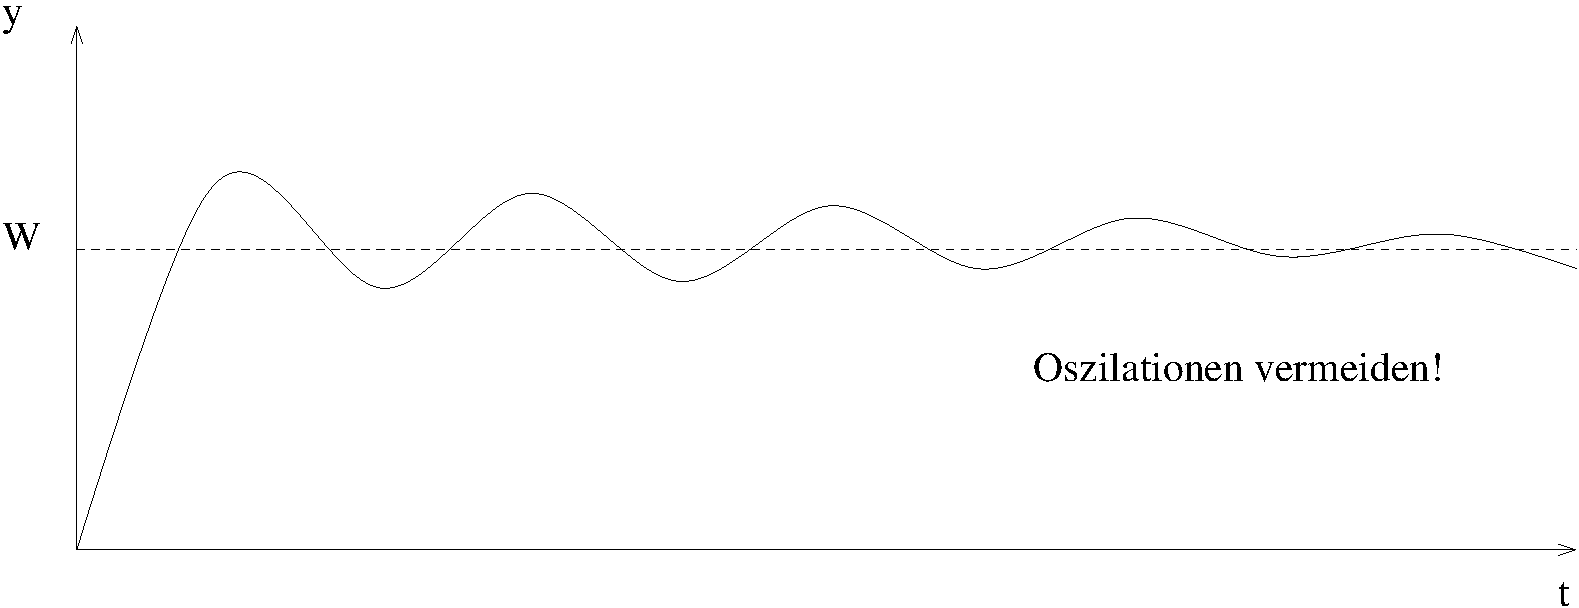
\includegraphics[width=.7\linewidth]{sysregel_No_3}
  \end{figure}
\begin{figure}[H]
\item[\RM{4}] \underline{Der Regelkreis muss hinreichend schnell sein}\\
  
    \centering
    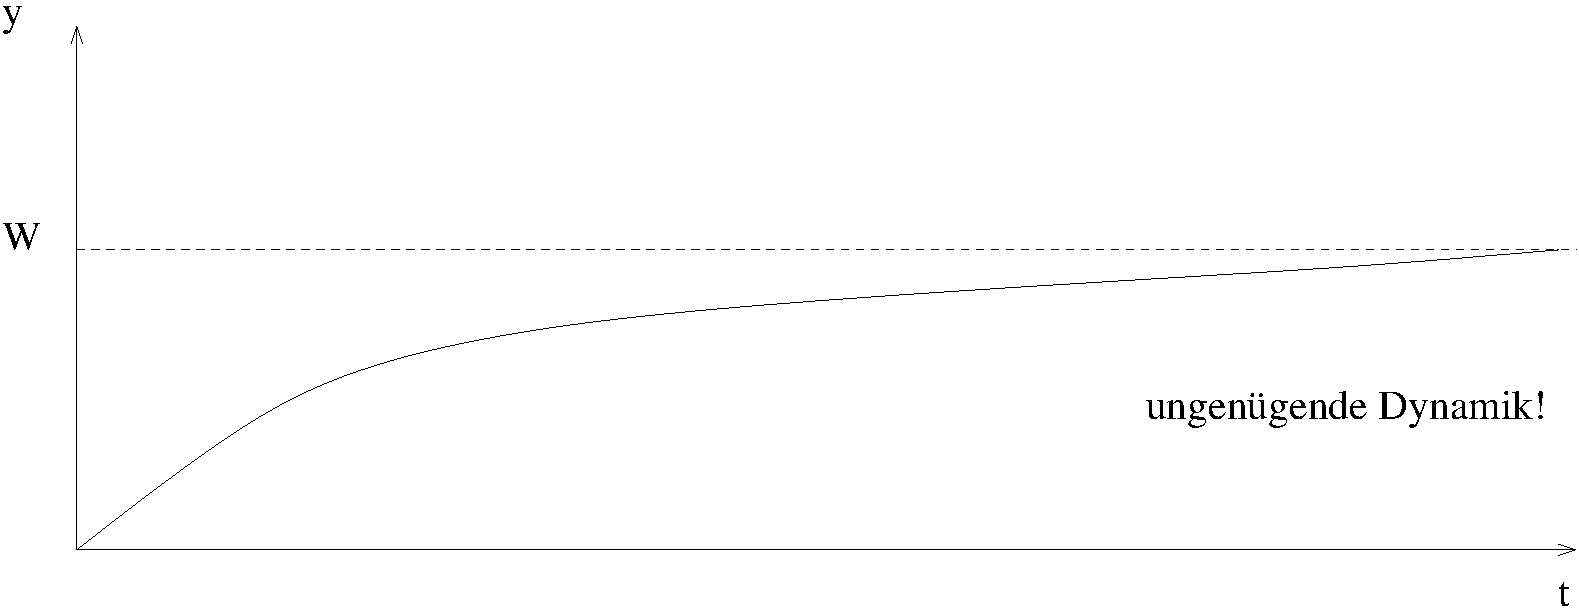
\includegraphics[width=.7\linewidth]{sysregel_No_4}
  \end{figure}

\end{itemize}
Auch (\RM{3}) und (\RM{4}) führen zu einem Zielkonflikt. Durch eine geeignete Korrektureinrichtung muss ein Kompromiss gefunden werden.

\subsubsection{Auswahl geeigneter Glieder zur dynamischen Korrektur}
\begin{figure}[H]
  \centering
  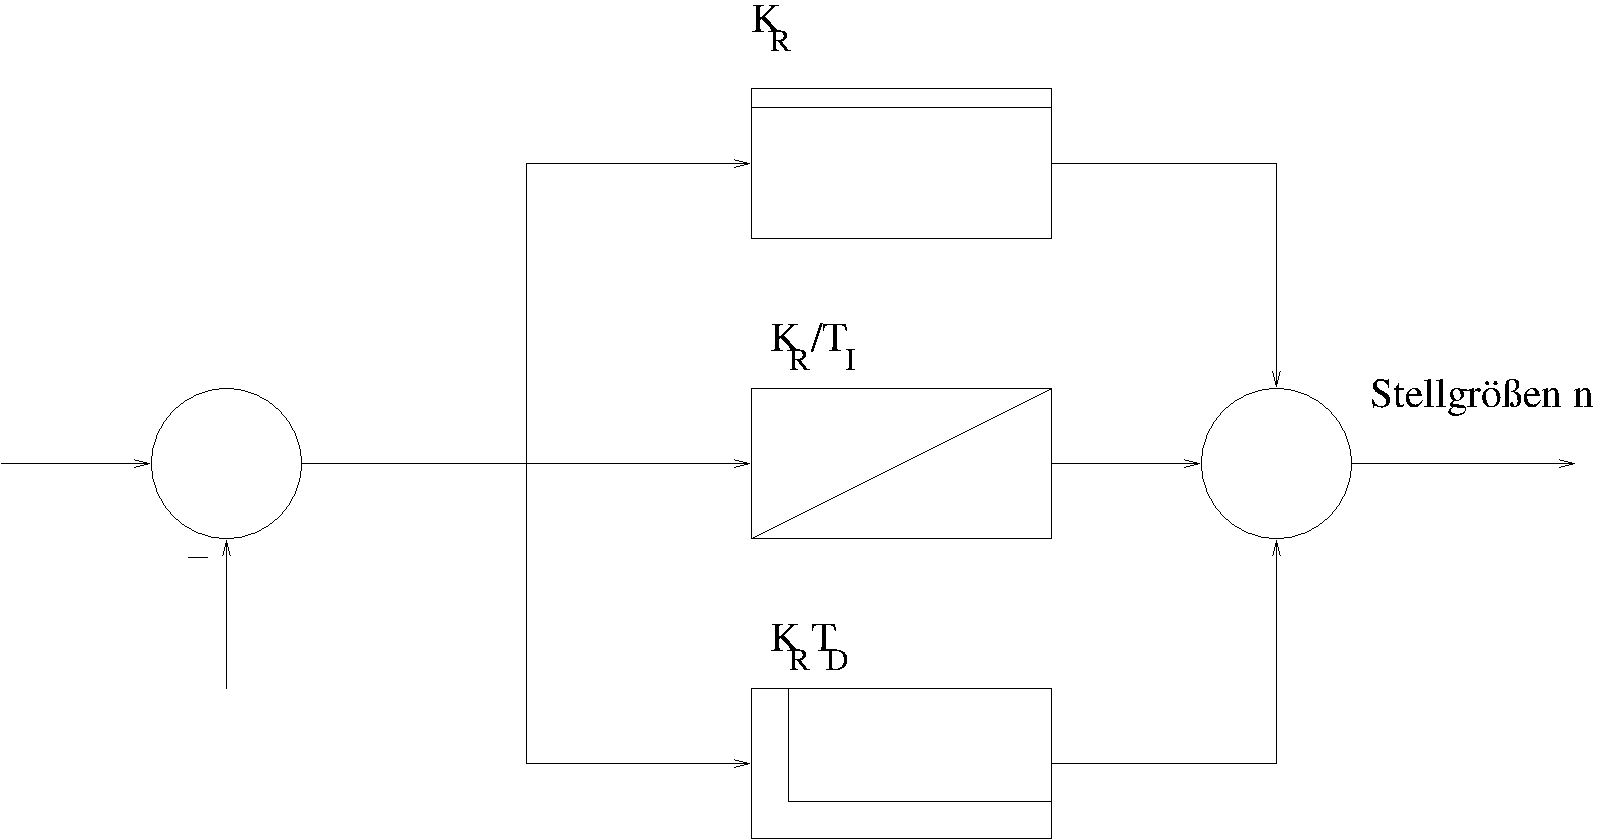
\includegraphics[width=.7\linewidth]{sysregel_No_2}
\end{figure}


\begin{description}
\item[R-Regler:] Je größer die Regeldifferenz, desto größer ist die Stellgröße
\item[I-Regler:] Lange andauernde Regeldifferenzen werden integriert, sodass die Stellgröße anwächst. Diese Regler sind \emph{stationär genau} nach Forderung \RM{2}
\item[D-Regler:] Sobald sich die Regeldifferenz ändert, wird eine Stellgröße erzeugt. Hier aus ergibt sich eine schnelle Reaktion nach Forderung \RM{4} 
\end{description}

\paragraph{Kombination: PID-Regler}

\begin{align*}
  \begin{array}{lllll}
    G_R(s)&=&K_R(1+\frac{1}{T_Is}+T_Ds)\\
    G_R(s)&=&\underbrace{\frac{K_R}{T_I}}_{u}\frac{1+T_Is+T_IT_Bs^2}{s}&=&u\cdot \frac{(1+T_1s)(1+T_2s)}{s}
  \end{array}
\end{align*}
mit $T_1>T_2$ und $T_1T_2=T_I+T_D$ sowie $T_1+T_2=T_I$\\
Dies ist schlecht realisierbar, da der Zählergrad=2>Nennergrad. Daher wird das System durch eine zusätzliche Zeitkonstante im Nenner zum ``realen PID-Regler'' erweitert:
\[
G_R(s)=\frac{K_R}{T_I}\frac{(1+T_1s)(1+T_2s)}{s(1+T_Ns)}
\] 
\textbf{Faustregel:} $T_N \approx \frac{1}{10}T_2$


\subsubsection{Reglersynthese auf Basis des Bodediagramms}

\begin{itemize}
\item Vorab für (\RM{2}):I-Anteil einführen, falls Strecke keinen eigenen I-Anteil besitzt.
\item für (\RM{1}):Stabilität nach dem Nyquist-Kriterium
\item Direkt an der Stabilitätsgrenze schwingt das System stark, daher wird der Regler in einem gewissen Abstand zu dieser Grenze dimensioniert. Es wird eine Phasenreserve $\Phi_R$ vorgegeben, um die Forderung (\RM{3}) zu erfüllen. Dadurch wird die Schwingung unterbunden, und Bauteiltoleranzen und Störungen führen nicht zu instabilitäten der Systems.
\end{itemize}
\begin{description}
\item[Faustregel:] $\Phi_R$ wird zwischen $30\degree$ und $70\degree$ gewählt. Je kleiner $\Phi_R$, desto mehr werden Schwingungen gedämpft. Allerdings wird der Regler mit zunehmendem $\Phi_R$ auch langsamer. Es muss also ein Kompromiss gefunden werden.\\
Die Durchtrittsfrequenz $\omega_D$ bestimmt die Dynamik (``Schnelligkeit'') des geregelten Systems. Daher ist die Dynamische Korrektur so zu wählen, dsas $\omega_D$ möglichst hoch liegt, um gute Dynamik zu erreichen (\RM{4})  
\end{description}
\begin{itemize}
\item z.B. PID-Regler zur dynamischen Korrektur (im Bodediagramm)
  \begin{figure}[H]
    \centering
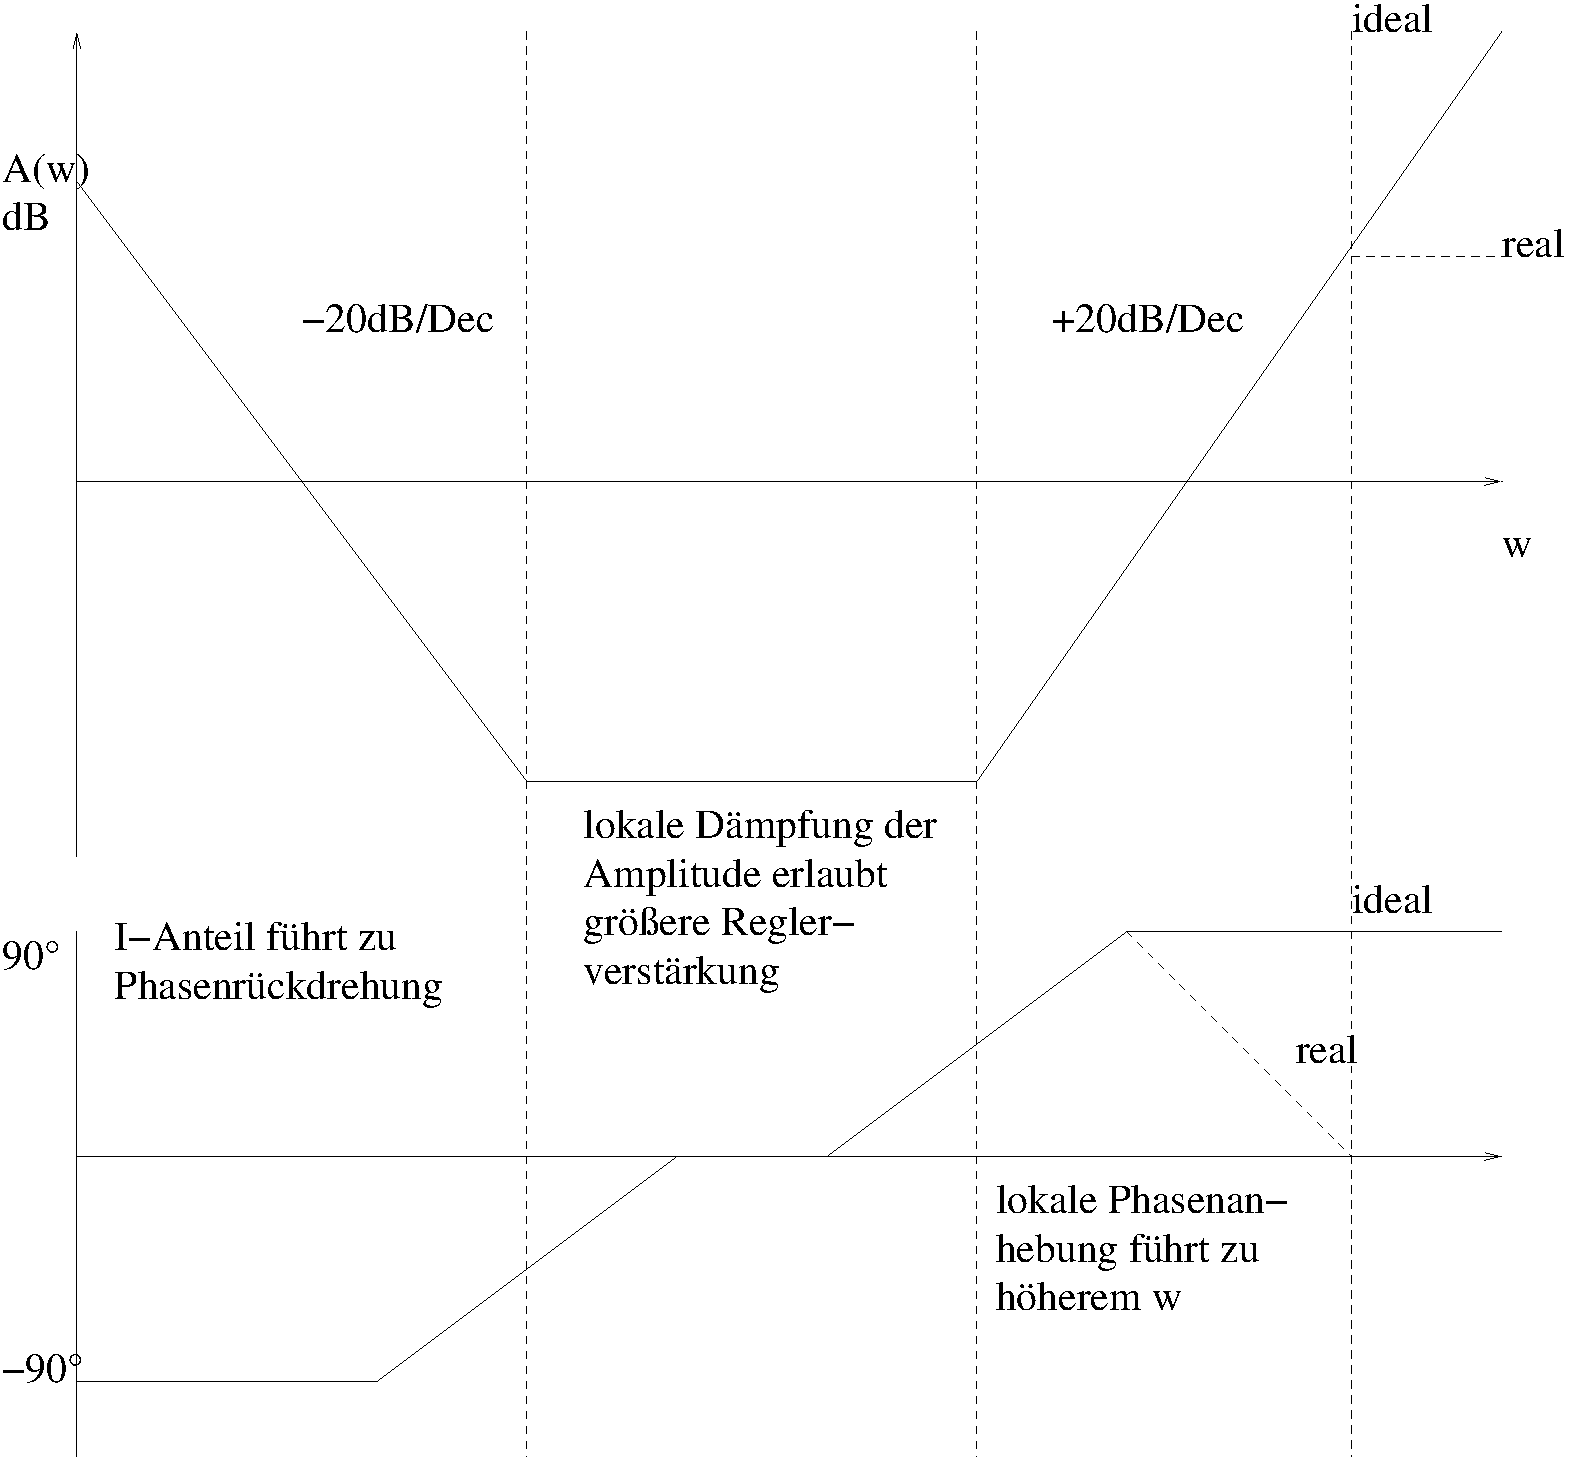
\includegraphics[width=.7\linewidth]{sysregel_PID}
  \end{figure}
\end{itemize}
\begin{description}
\item[Alternatives Vorgehen:] Reglerzeitkonstanten so wählen, dass die größten Zeitkonstanten (dynamisch dominant) der Strecke kompensiert werden. 
\end{description}
\begin{bsp} 
\end{bsp}
Strecke aus dem vorhergehenden Beispiel:
\[
G_s(s)=\frac{0.1}{(1+10s)(1+5s)(1+2s)}
\]
\begin{itemize}
\item Strecke ist stabil \checkmark
\item Strecke hat keinen I-Anteil $\rightarrow$ PID-Regler verwenden (real)
\item Reglerzeitkonstanten sollen Streckenzeitkonstanten kompensieren
\end{itemize}

\begin{figure}[H]
  \centering
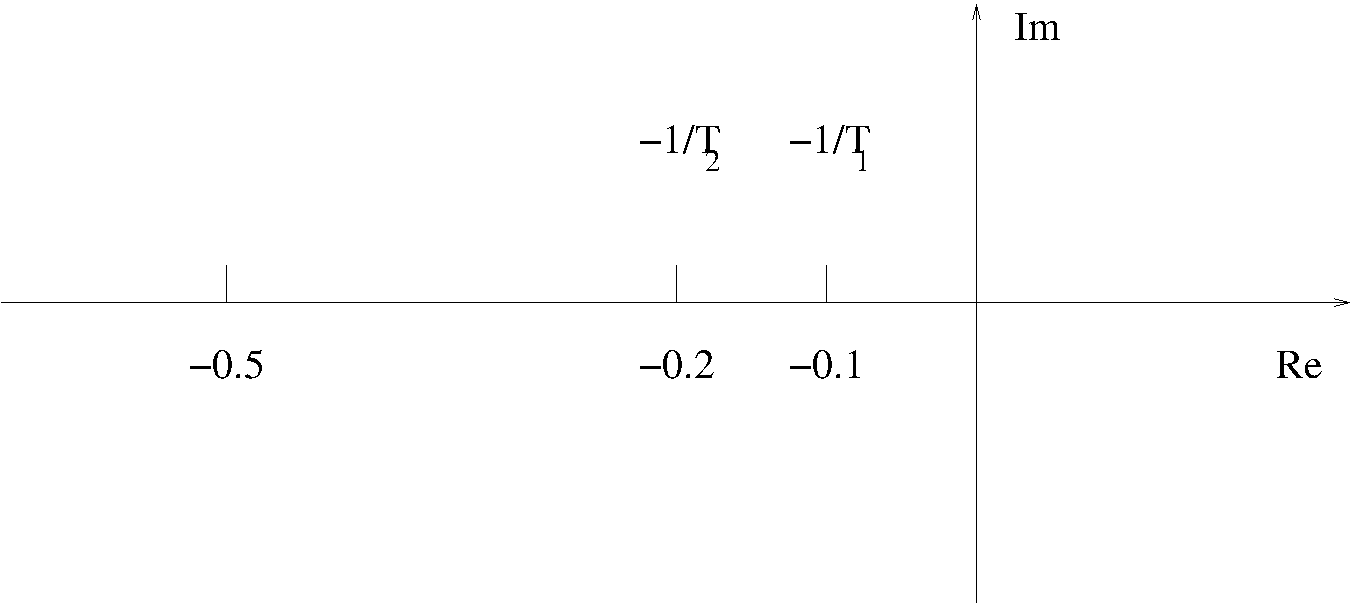
\includegraphics[width=0.7\linewidth]{sysregel_bsp_5_4}  
\end{figure}
\begin{align*}
  \begin{array}{lllll}
  G_0(s)&=&G_R(s)\cdot G_s(s)&=&v \cdot \frac{(1+T_1s)(1+T_2s)}{s(1+T_ns} \cdot \frac{0.1}{(1+10s)(1+5s)(1+2s)} \\
&=&v\cdot \frac{\cancel{(1+10s)}\cancel{(1+5s)}\cdot 0.1}{s\cdot \cancel{(1+10s)}\cancel{(1+5s)}(1+2s)(1+0.5s)}&=&\frac{v\cdot 0.1}{\underbrace{s}_{I}\underbrace{(1+2s)}_{1. PT_1}\underbrace{(1+0.5s)}_{2. PT_1}}
  \end{array}
\end{align*}

\paragraph{Bodediagramm für v=1}

\begin{figure}[H]
  \centering
  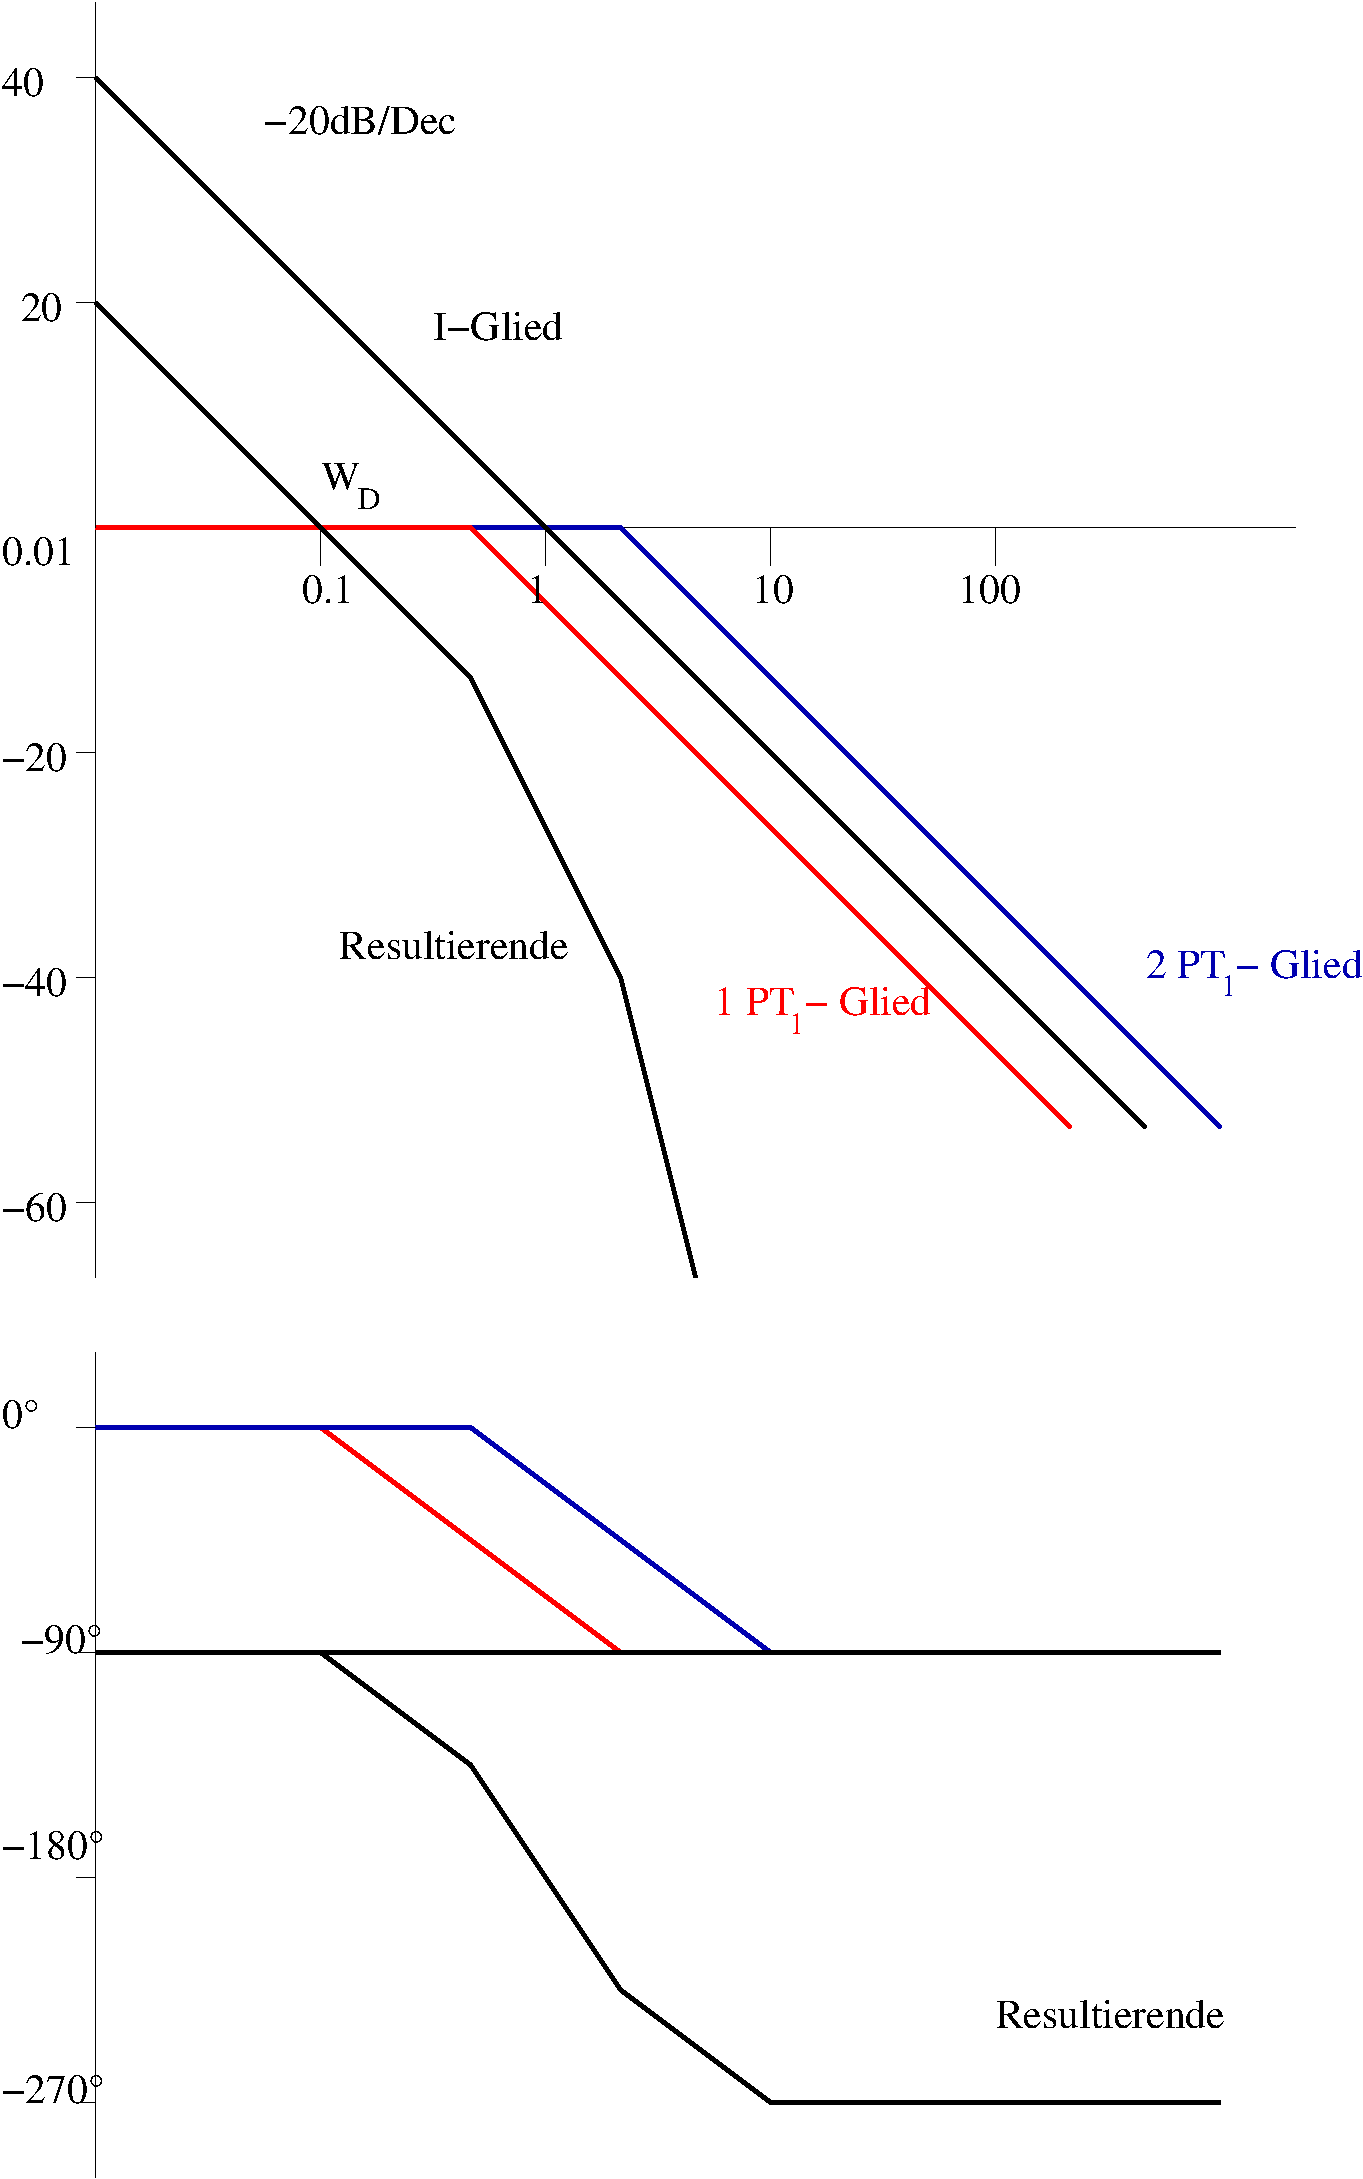
\includegraphics[width=.7\linewidth]{sysregel_bode_5-4}
\end{figure}
Man erkennt, dsas bei $\Phi_R=40\degree \omega_D=0.5$ ist. Damit $ \omega_D$ die Durchtrittsfrequenz ist (Schnitt mit 0~dB) kann die Ampliture um ca. 14~dB verschoben werden. ($\rightarrow v\approx 7)$. Damit ist der PID-Regler definiert als:
\[
G_R(s)=7\cdot \frac{1+10s)(1+5s)}{s(1+0.5s)}
\]
\end{document}


 %ENDE DES ZU ERZEUGENDEN DOKUMENTES! AB HIER WIRD BEI DER DOKUMENTERSTELLUNG ALLES IGNORIERT!!
